%%
%% This is file `article1.tex', % generated with the docstrip utility.
%%
%% The original source files were:
%%
%% dms.dtx  (with options: `article') % Example TeX file for the documentation %
%of the jurabib package % Copyright (C) 1999, 2000, 2001 Jens Berger % See
%dms.ins  for the copyright details.
%% 
%%% ====================================================================
%%%  @LaTeX-file{ %%     filename        = "dms.dtx", %%     author    =
%"Nicolas Beauchemin, Damien Rioux-Lavoie, Victor Fardel, Jonathan Godin", %%
%copyright = "Copyright (C) 2000 , DMS %%                  all rights reserved.
%Copying of this file is %%                  authorized only if either: %%
%(1) you make absolutely no changes to your copy, %%                  including
%name; OR %%                  (2) if you do make changes, you first rename it %%
%to some other name.", %%     address   = "Département de Mathématiques et de
%Statistique", %%     telephone = "514-343-6705", %%     FAX       =
%"514-343-5700", %%     email     = "aide@dms.umontreal.ca (Internet)", %%
%keywords  = "latex, amslatex, ams-latex, theorem", %%     abstract  = " Ce
%fichier est un package conçu pour être %%                  utilisé avec la
%version de LaTeX2e 1995/06/01. Il %%                  est prévue pour la classe
%``amsbook''. Il en %%                  modifie le format des pages, l'entête
%des %%                  sections, etc, afin d'être  conforme au modèle de %%
%mémoire de maîtrise de l'Université de %%                  Montréal. Finalement
%ce fichier est grandement %%                  inspiré du fichier
%amsclass.dtx.", %%     docstring = "The checksum field contains: CRC-16
%checksum, %%                  word count, line count, and character count, as
%%%                  produced by Robert Solovay's checksum utility."}
%%%  ====================================================================


%% To change chapter header dynamically from french to english, use
%%\entetedynamique
\setcounter{corA}{0} % Pour recommancer à compter les def,
                     % theo, etc. à partir de 1
 % Pour écrire un article en français
%% \francais
 % Pour écrire un article en anglais
\anglais
%% NOTE: La plupart des macros ont un nom en anglais. % P.ex. \adresse et
%\address fonctionnent et sont équivalents. % \revue=\journal % \auteur=\author
%% \titre=\title

\doublespacing

%% Les contributions apparaîtront habituellement après % \maketitle (voir un peu
%plus bas). Selon les goûts, il est % possible de mettre les contributions %
%avant la page titre de l'article, simplement en les écrivant % directement ici.
%Par exemple :
 % \cleardoublepage \pdfbookmark[chapter]{Contributions}{contrib1} % Remplacer
 % par contrib2 pour l'article 2 etc. {\bfseries\Large\noindent Contributions de
 % <mon nom> et rôle joué par les coauteurs} J'ai contribué en...
 %
 % Le rôle des coauteurs a été de...

%% Nom de la revue de publication
\revue{Frontiers in Ecology and Evolution and can be found at https://doi.org/10.3389/fevo.2021.623141}
\article{SVD Entropy reveals the high complexity of ecological networks}\label{SVD}
%% On peut se référer aux numéros de chapitre ou d'article comme suit. % Si on
%fait % \label{chap:article1}, % alors \ref{chap:article1} donnera le numéro du
%chapitre. On peut ensuite faire % \labelart{art:article1} % et alors
%\ref{art:article1} donnera le numéro d'article. % Par exemple, si cette article
%est le premier article et le deuxième chapitre, % alors si on écrit % Voir le
%chapitre~\ref{chap:article1} (l'article~\ref{art:article1}). % deviendra % Voir
%le chapitre 2 (l'article 1). % Si on veut écrire « premier article » au lieu «
%article 1 », on peut % simplement faire % \ordinal{\ref{art:article1}}~article
%% devient première article % ou % \Ordinal{\ref{art:article1}}~article  %
%devient Première article (avec la majuscule) % Si on est en mode \anglais,
%\ordinal écrire first, second,...

%%%%%%%%%%%%%%%%%%%%%%%%%%%%%%%%%%%%%%%%%%%%%%%%%%%%%%%%%%%%%%%
%%%%%%%%%%%%%%%%%     Contribution     %%%%%%%%%%%%%%%%%%%%%%%% %%%%%%%%%%%%%%%%
%(lire attentivement) %%%%%%%%%%%%%%%%%%%%%%%%
%%%%%%%%%%%%%%%%%%%%%%%%%%%%%%%%%%%%%%%%%%%%%%%%%%%%%%%%%%%%%%%
 % Contribution(s) peronnelle(s) à l'article et rôle joué par tous les
 % coauteur·e·s
 %
 % Nécessaire seulement lorsque vous n'êtes pas seul·e auteur·e. Les
 % contributions peuvent apparaître ailleur dans la thèse. Si \contributions est
 % laissé vide (p.ex. si vous effacez celui ci-bas), aucune contributions ne
 % seront générées sur la page titre de l'article. Vous pouvez alors mettre un
 % \newpage si vous souhaitez que les résumé et abstract soient sur la page
 % suivante.
 %
 % REMARQUE : À peu près toutes les constructions \LaTeX\ sont permises dans les
 % contributions.
 %
 % La commande admet une option [<entête>]
\contributions%[Mes contributions et le rôle des coauteurs]
{ 

TP and TS designed the study and edited the manuscript for submission. TS performed the analysis and wrote the manuscript. All authors contributed to the article and approved the submitted version.\\[1cm]
}

%%% INFORMATIONS POUR LA PAGE TITRE
 % Premier auteur·e et adresse

\auteur{Tanya Strydom}
\adresse{Département de Sciences Biologiques, Université de Montréal, Montreal, QC, Canada\\ Québec Centre for Biodiversity Sciences, Montreal, QC, Canada}
\auteur{Giulio V. Dalla Riva}
\adresse{School of Mathematics and Statistics, University of Canterbury, Christchurch, New Zealand}
\auteur{Timothée Poisot}
\adresse{Département de Sciences Biologiques, Université de Montréal, Montreal, QC, Canada\\ Québec Centre for Biodiversity Sciences, Montreal, QC, Canada}
%

\maketitle

\begin{resume}{décomposition en valeurs singulières, complexité physique, réseau bipartite, entropie, pollinisation, analyse de réseaux écologiques} Quantifier la complexité des réseaux écologiques reste difficile à évaluer. Principalement, la complexité a été définie sur la base de la complexité structurelle (ou comportementale) du système. Ces définitions ignorent la notion de « complexité physique », qui peut mesurer la quantité d’informations contenues dans un réseau écologique et la difficulté de les compresser. Nous présentons respectivement le déficit de rang relatif et l’entropie SVD comme mesures de la complexité "externe" et "interne". En utilisant des réseaux écologiques bipartites, nous constatons qu’ils présentent tous une complexité physique très élevée, presque maximale. Les réseaux de pollinisation, en particulier, sont plus complexes que d’autres types d’interactions. De plus, nous constatons que l'entropie SVD est liée à d'autres mesures structurelles de complexité (imbrication, connectivité et rayon spectral), mais ne renseigne pas sur la résilience d'un réseau lors de l'utilisation de cascades d'extinction simulées, ce qui a déjà été rapporté pour des mesures structurelles de complexité. Nous soutenons que l’entropie SVD fournit une mesure fondamentalement plus "correcte" de la complexité des réseaux et devrait être ajoutée à la boîte à outils des descripteurs des réseaux écologiques à l’avenir.
\end{resume}

\begin{abstract}{singular value decomposition, physical complexity, bipartite network, entropy, pollination, ecological network analysis} Quantifying the complexity of ecological networks has remained elusive. Primarily, complexity has been defined on the basis of the structural (or behavioural) complexity of the system. These definitions ignore the notion of “physical complexity,” which can measure the amount of information contained in an ecological network, and how difficult it would be to compress. We present relative rank deficiency and SVD entropy as measures of “external” and “internal” complexity, respectively. Using bipartite ecological networks, we find that they all show a very high, almost maximal, physical complexity. Pollination networks, in particular, are more complex when compared to other types of interactions. In addition, we find that SVD entropy relates to other structural measures of complexity (nestedness, connectance, and spectral radius), but does not inform about the resilience of a network when using simulated extinction cascades, which has previously been reported for structural measures of complexity. We argue that SVD entropy provides a fundamentally more “correct” measure of network complexity and should be added to the toolkit of descriptors of ecological networks moving forward.
\end{abstract}

\begin{refsection}

\section{Introduction}

Ecologists have turned to network theory because it offers a powerful
mathematical formalism to embrace the complexity of ecological communities
(\cite{Bascompte2007PlaMut}). Indeed, analysing ecological systems as networks
highlighted how their structure ties into ecological properties and processes
(\cite{Proulx2005NetThi, Poulin2010NetAna}), and there has been a subsequent
explosion of measures that purport to capture elements of network structure, to be related to the ecology of the system they describe (\cite{Delmas2018Analysing}). Since the early days of network ecology, ecological networks have been called
``complex''. This sustained interest for the notion of complexity stems, in
part, from the strong ties it has to stability (\cite{Landi2018Complexity}). As such,
many authors have looked for clues, in the network structure, as to why the
networks do not collapse (\cite{Borrelli2015SelIns, Staniczenko2013GhoNes,
Gravel2016StaCom, Brose2006AllSca}). Yet decades of theoretical refinements on
the relationship between complexity and stability had a hard time when
rigorously tested on empirical datasets (\cite{Jacquet2016NoCom}); although
ecological networks may be complex, our current measures of complexity do not
translate into predictions about stability.

Surprisingly, \emph{complexity} itself has proven an elusive concept to define
in a rigorous way. It has over time been defined as connectance
(\cite{Rozdilsky2001ComCan}), as measures of the diversity of species or their
interactions (\cite{Landi2018Complexity}), or as a combination of species richness and trophic diversity (\cite{Duffy2007FunRol}). In short, network ecology as a field readily assumes that because we have more information about a system, or because this system has more components, or simply because this system can be expressed as a network, it follows that the system is complex. But such a diversity of definitions, for a concept that is so central to our quest to understand network stability, decreases the clarity of what complexity means, and what all of these alternative definitions do actually capture. This is a common thread in some measures of ecological network structure, as has been discussed at length for
the various definitions of nestedness (\cite{Ulrich2009ConSG}).

None of the previous definitions of complexity are formally wrong, in that they do capture an aspect of complexity that ultimately ties to the behaviour of the system, \emph{i.e.,} its low predictability over time. Yet
(\cite{Adami2002WhaCom}) provides a compelling argument for why the
complexity of the behaviour does not necessarily reflects the complexity of the
system; in fact, one would be very hard pressed to think of a more simple system
than the logistic map used by \cite{May1976SimMat} to illustrate how easily
complexity of behaviour emerges. Rather than yielding to the easy assumption
that a system will be complex because it has many parts, or because it exhibits
a complex behaviour, \cite{Adami2002WhaCom} suggests that we focus on
measuring ``physical complexity'', \emph{i.e.,} the amount of information
required to encode the system, and how much signal this information contains.
Complex systems, in this perspective, are those who cannot easily be compressed
- and this is a notion we can explore for the structure of ecological networks.

Ecological networks are primarily represented by their adjacency matrices,
\emph{i.e.,} a matrix in which every entry represents a pair of species, which
can take a value of 1 when the two species interact, and a value of 0 when they
do not. These matrices (as any matrices) can easily be factorised using Singular
Value Decomposition (\cite{Forsythe1967ComSol, Golub1971SinVal}), which offers two
interesting candidate measures of complexity for ecological networks (both of
which we describe at length in the methods). The first measure is the rank of
the matrix, which works as an estimate of ``external complexity'', in that it
describes the dimension of the vector space of this matrix, and therefore the
number of linearly independent rows (or columns) of it. From an ecological
standpoint, this quantifies the number of unique ``strategies'' represented in
the network: a network with two modules that are distinct complete graphs has a
rank of 2. The second measure is an application of the entropy measure of
\cite{Shannon1948MatThe} to the non-zero singular values of the matrix
obtained through SVD. This so-called SVD entropy measures the extent to which
each rank encodes an equal amount of information, as the singular values capture
the importance of each rank to reconstruct the original matrix; this approach
therefore serves as a measure of ``internal complexity''.

In this manuscript, we present and evaluate the use of both the rank and SVD
entropy of ecological networks as alternative and more robust measures of
complexity when compared to traditional approaches to defining complexity. This
is done by using a collection of 220 bipartite networks from various types of
interaction, sizes, connectances, and environments. We show that while the rank
of the adjacency matrix holds little information, SVD entropy functions as an
appropriate quantification of the complexity of ecological systems. Notably, SVD
entropy is an intuitive, robust, non-structural approach to defining the
(surprisingly high) complexity of ecological networks, by relating them to their
`physical' as opposed to `behavioural' complexity. In this process we showcase a
breakdown in the assumption that all measures of complexity of networks are
indicative of their robustness to extinctions. Finally, we show that, despite
their high complexity, observed networks are less complex when compared to
pseudo-random networks, especially for larger networks. We propose that taking a
physical approach to quantifying the complexity of ecological networks is a step
in the right direction to unifying how we define complexity in the context of
ecological networks, as it restores other measures (like connectance and
nestedness) to their original role and signification.

\section{Data and methods}\label{data-and-methods}

We used all bipartite networks contained in the \texttt{web-of-life.es}
database. This database extracted species interaction networks from
supplementary materials across all inhabited continents and covers a large array
of sampling years, environments, organisms, and sampling methodologies. As such,
this dataset is particularly suited to describe general trends across \emph{all}
ecological networks. We specifically worked on the version of this dataset
distributed with the \texttt{EcologicalNetworks.jl} package
(\cite{Poisot2019EcoJl}) for the \emph{Julia} (\cite{Bezanson2017Julia})
programming language, in which all analyses were conducted. Using bipartite
networks means that interacting species are split into two sets (or interacting
groups) and along different dimensions in the interaction matrix. Thus, columns
in the matrix represent one group (or type) of species and rows represent the
other group of species involved in the interaction. Because SVD gives similar
results on the matrix and its transpose, it captures the complexity of both
sides of the system at once. A summary of the dataset is given in
\autoref{table:summary}.

\begin{table}[h!]
\centering
\begin{tabular}{||c c c c c||} 
 \hline
 Interaction type & Sample size & Latitude range & Richness (top) & Richness
 (bottom) \\ [0.5ex] \hline\hline
 Host-Parasite & 51 & 38.77 \(\rightarrow\) 72.65 & 20.47 & 12.23 \\ 
 Plant-Ant & 4 & -16.11 \(\rightarrow\) -2.40 & 18.75 & 21.75 \\
 Plant-Herbivore & 4 & 30.20 \(\rightarrow\) 64.91 & 49.5 & 29.25 \\
 Pollination & 134 & -43.09 \(\rightarrow\) 81.81 & 40.22 & 18.02 \\
 Seed Dispersal & 33 & -28.95 \(\rightarrow\) 53.05 & 18.75 & 25.12 \\ [1ex] 
 \hline
\end{tabular}
\caption{Overview of the \texttt{web-of-life.es} dataset. We used all networks
with up to 500 species. Although there are spatial biases in the sampling of
interaction types (and some interaction types being under-represented), this
dataset covers a range of latitudes from -43 degrees south to 81 degrees north.
The average richness of the top and bottom level of the bipartite networks are
also given in the last columns.}
\label{table:summary}
\end{table}

\subsection{Estimating complexity with rank
deficiency}\label{estimating-complexity-with-rank-deficiency}

The rank of \(\mathbf{A}\) (noted as \(r = \text{rk}(\mathbf{A})\)) is the
dimension of the vector space spanned by the matrix and corresponds to the
number of linearly independent rows or columns; therefore, the maximum rank of a
matrix (\(M = \text{rk}_{\text{max}}(\mathbf{A})\)) will always be equal to the
length of the shortest dimension of \(\mathbf{A}\), which ecologically speaking
is the richness of the least species-rich compartment of the bipartite network
(or the richness in the case of unipartite networks). A matrix is
``full-ranked'' when \(r=M\), \emph{i.e.,} all of its rows/columns are unique.
Matrices that are not full-ranked are called rank deficient, and we can measure
rank deficiency using \(d = M-r\). So as to control for the difference in
species richness of the different networks, we report the relative rank
deficiency, \emph{i.e.,} expressed as a ratio between rank deficiency and the
maximal rank:

\[D = 1-\frac{r}{M}\]\

This measure returns values between 0 (the matrix is full ranked) and \(1-M^{-1}
\approx 1\) (the matrix has rank 1). This serves as a coarse estimate of
complexity, as the more unique columns/rows are in the matrix, the larger this
value will be. Yet it may also lack sensitivity, because it imposes a stringent
test on uniqueness, which calls for more quantitative approaches to complexity.

\subsection{Estimating complexity with SVD
entropy}\label{estimating-complexity-with-svd-entropy}

Singular Value Decomposition (SVD) is the factorisation of a matrix
\(\mathbf{A}\) (where \(\mathbf{A}_{m,n} \in\mathbb{B}\) in our case, but SVD
works for matrices of real numbers as well) into the form
\(\mathbf{U}\cdot\mathbf{\Sigma}\cdot \mathbf{V}^T\). Where \(\mathbf{U}\) is an
\(m \times m\) orthogonal matrix and \(\mathbf{V}\) an \(n \times n\) orthogonal
matrix. The columns in these matrices are, respectively, the left- and
right-singular vectors of \(\mathbf{A}\), were \(\mathbf{U} =
\mathbf{A}\mathbf{A}^T\) and \(\mathbf{V} = \mathbf{A}^T\mathbf{A}\).
\(\mathbf{\Sigma}\) is a matrix that only contains non-negative \(\sigma\)
values along its diagonal and all other entries are zero. Where \(\sigma_{i} =
\Sigma{ii}\), which contains the singular values of \(\mathbf{A}\). When the
values of \(\mathbf{\sigma}\) are arranged in descending order, the singular
values (\(\mathbf{\Sigma}\)) are unique, though the singular vectors
(\(\mathbf{U}\) and \(\mathbf{V}\)) may not be.

After the Eckart-Young-Mirsky theorem (\cite{Eckart1936AppOne, Golub1987GenEck}),
the number of non-zero entries (after rounding of small values if required due
to numerical precision issues in computing the factorisation) in
\(\mathbf{\sigma}\) is the rank of matrix \(\mathbf{A}\). For the sake of
simplicity in notation, we will use \(k = \text{rk}(\mathbf{A})\)) for the rank
of the matrix. Because only the first \(k\) elements of \(\mathbf{\sigma}\) are
non-zero, and that the result of the SVD is a simple matrix multiplication, one
can define a truncated SVD containing only the first \(k\) singular values.

Intuitively, the singular value \(i\) (\(\sigma_i\)) measures how much of the
dataset is (proportionally) explained by each vector - therefore, one can
measure the entropy of \(\mathbf{\sigma}\) following \cite{Shannon1948MatThe}. High
values of SVD entropy reflects that all vectors are equally important,
\emph{i.e.,} that the structure of the ecological network cannot efficiently be
compressed, and therefore indicates high complexity (\cite{Gu2016HowLon}). Because
networks have different dimensions, we use Pielou's evenness
(\cite{Pielou1975EcoDiv}) to ensure that values are lower than unity, and quantify
SVD entropy, using \(s_i = \sigma_i/\text{sum}(\sigma)\) as:

\[J = -\frac{1}{\ln(k)}\sum_{i=1}^k s_i\cdot\ln(s_i)\]\

\section{Results and discussion}\label{results-and-discussion-svd}

\subsection{Most ecological networks are close to
full-rank}\label{most-ecological-networks-are-close-to-full-rank}

The majority (63\% of our dataset) of bipartite ecological networks have a
relative rank deficiency of 0 (\autoref{fig:size}), which indicates that all
species have different and unique interaction lists. Interestingly, the networks
that had a comparatively larger relative rank deficiency tended to be smaller
ones. Yet because most of the networks return the same value, matrix rank does
not appear to be a useful or discriminant measure of network complexity. Another
striking result (from \autoref{fig:size}) is that the SVD entropy of ecological
networks is really large -- although the value can range from 0 to 1, all
ecological networks had SVD entropy larger than 0.8, which is indicative of a
strong complexity.

\begin{figure}[h]
    \centering
    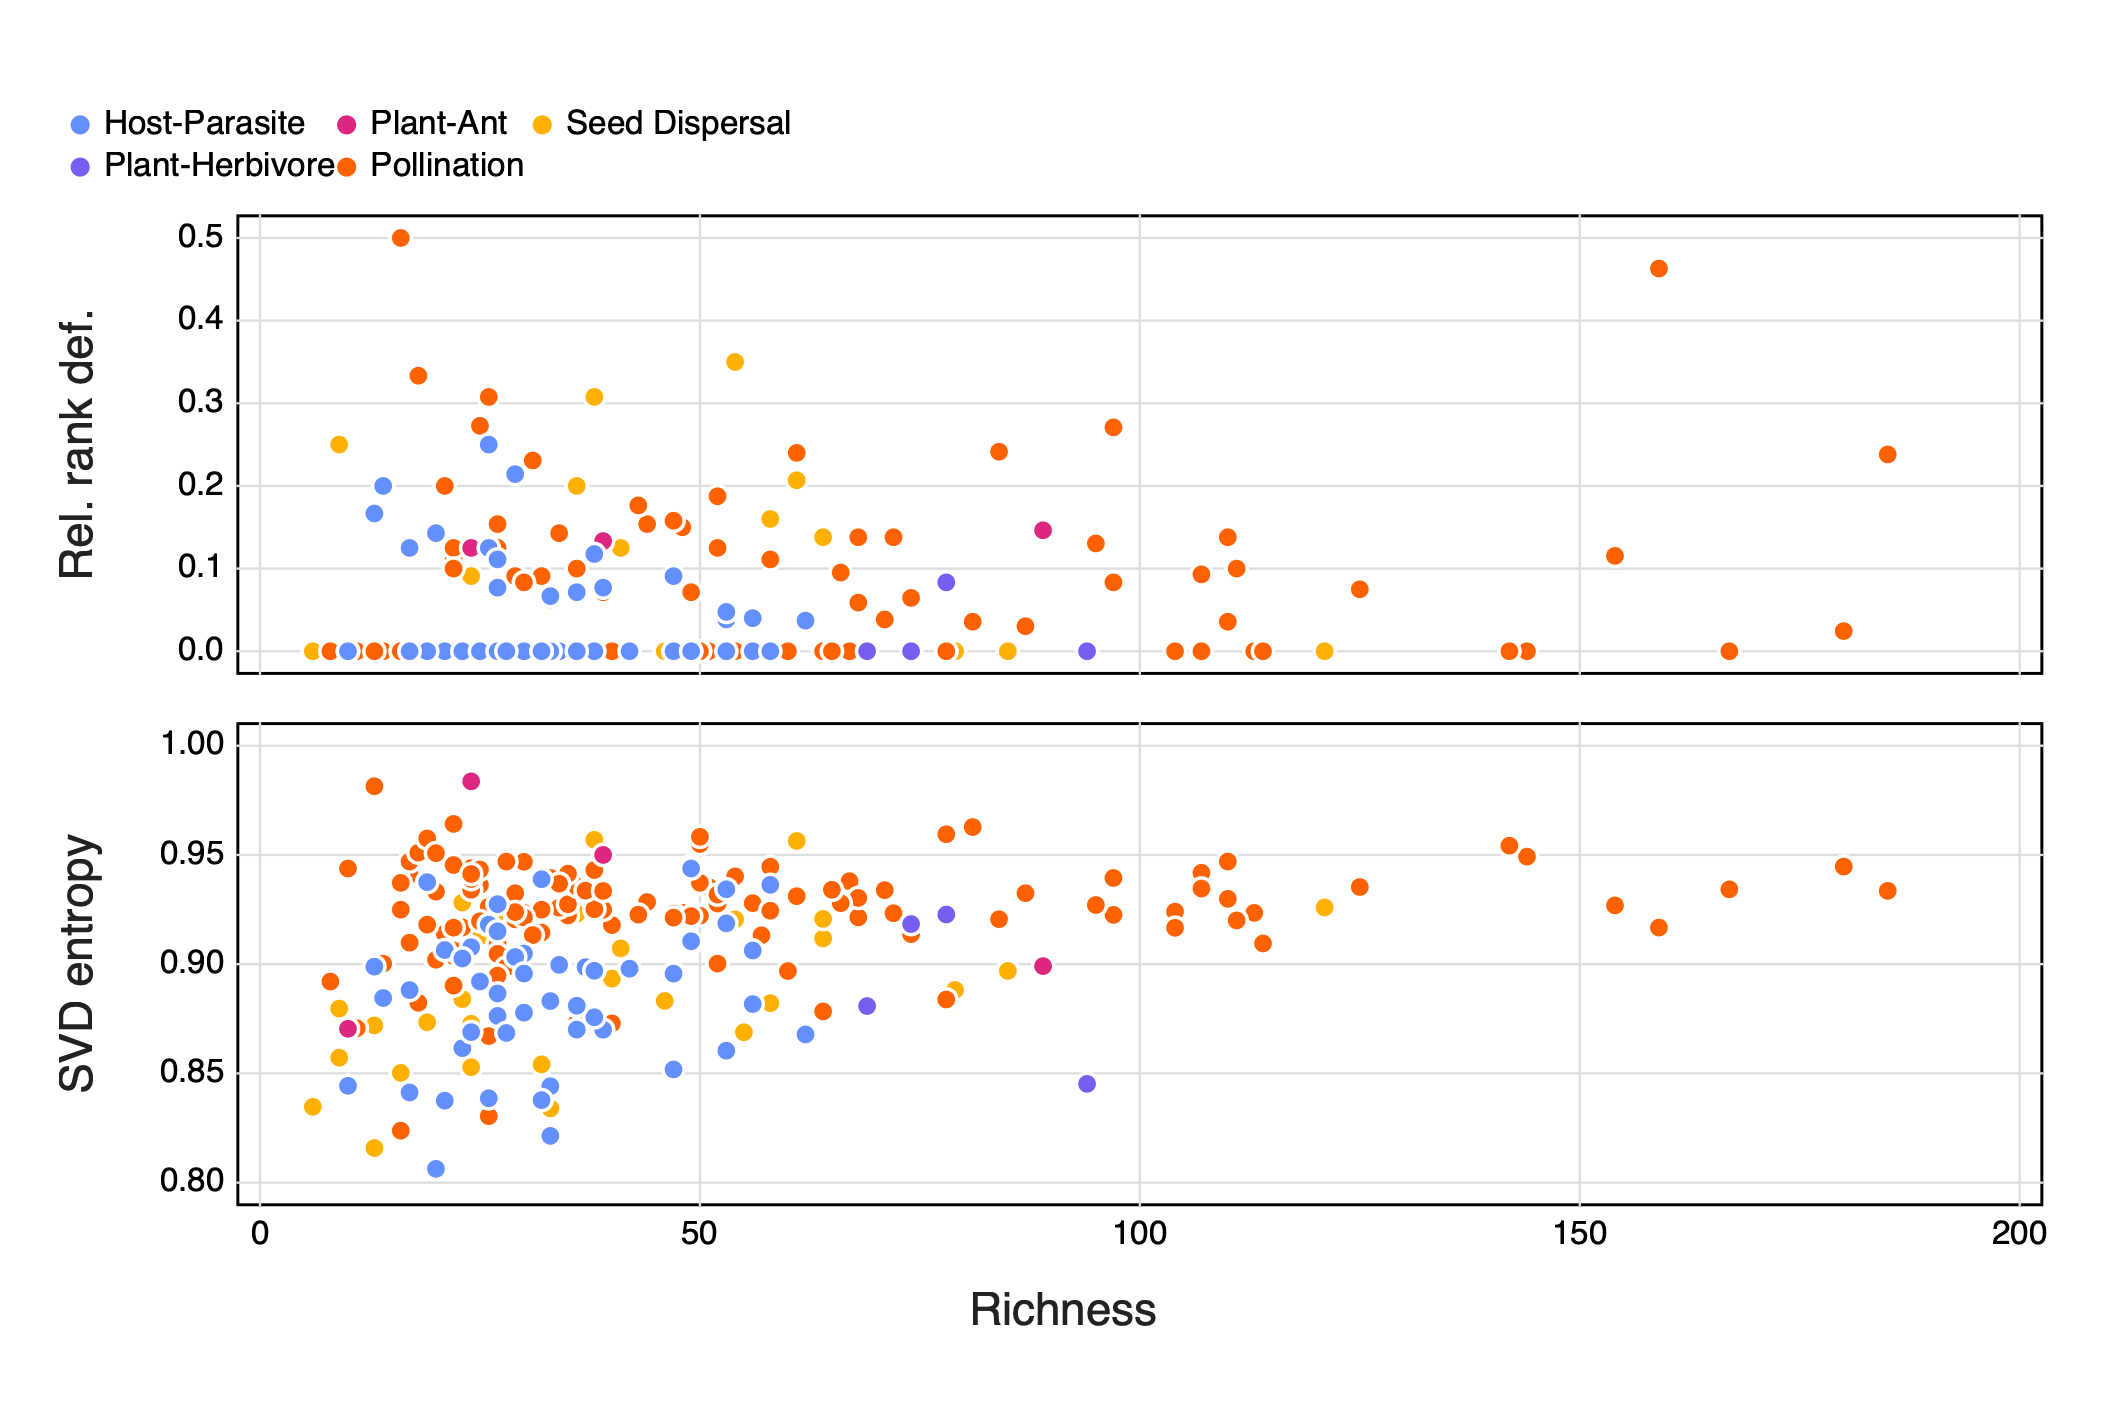
\includegraphics[width=\textwidth]{figures/size_v_rankentropy.png}
    \caption{The relationship between network richness and relative rank
deficiency, and SVD entropy. The different types of interactions are indicated
by the colours.}
    \label{fig:size}
\end{figure}

As expected following the observation that ecological networks are
overwhelmingly full ranked, we do not see a relationship between SVD entropy and
relative rank deficiency, neither do we observe differences between interaction
types (\ref{fig:entropy_v_rank}). Based on these results, we feel confident that
SVD entropy provides a more informative measure of the complexity of ecological
networks, and will use it moving forward.

\begin{figure}[h]
    \centering
    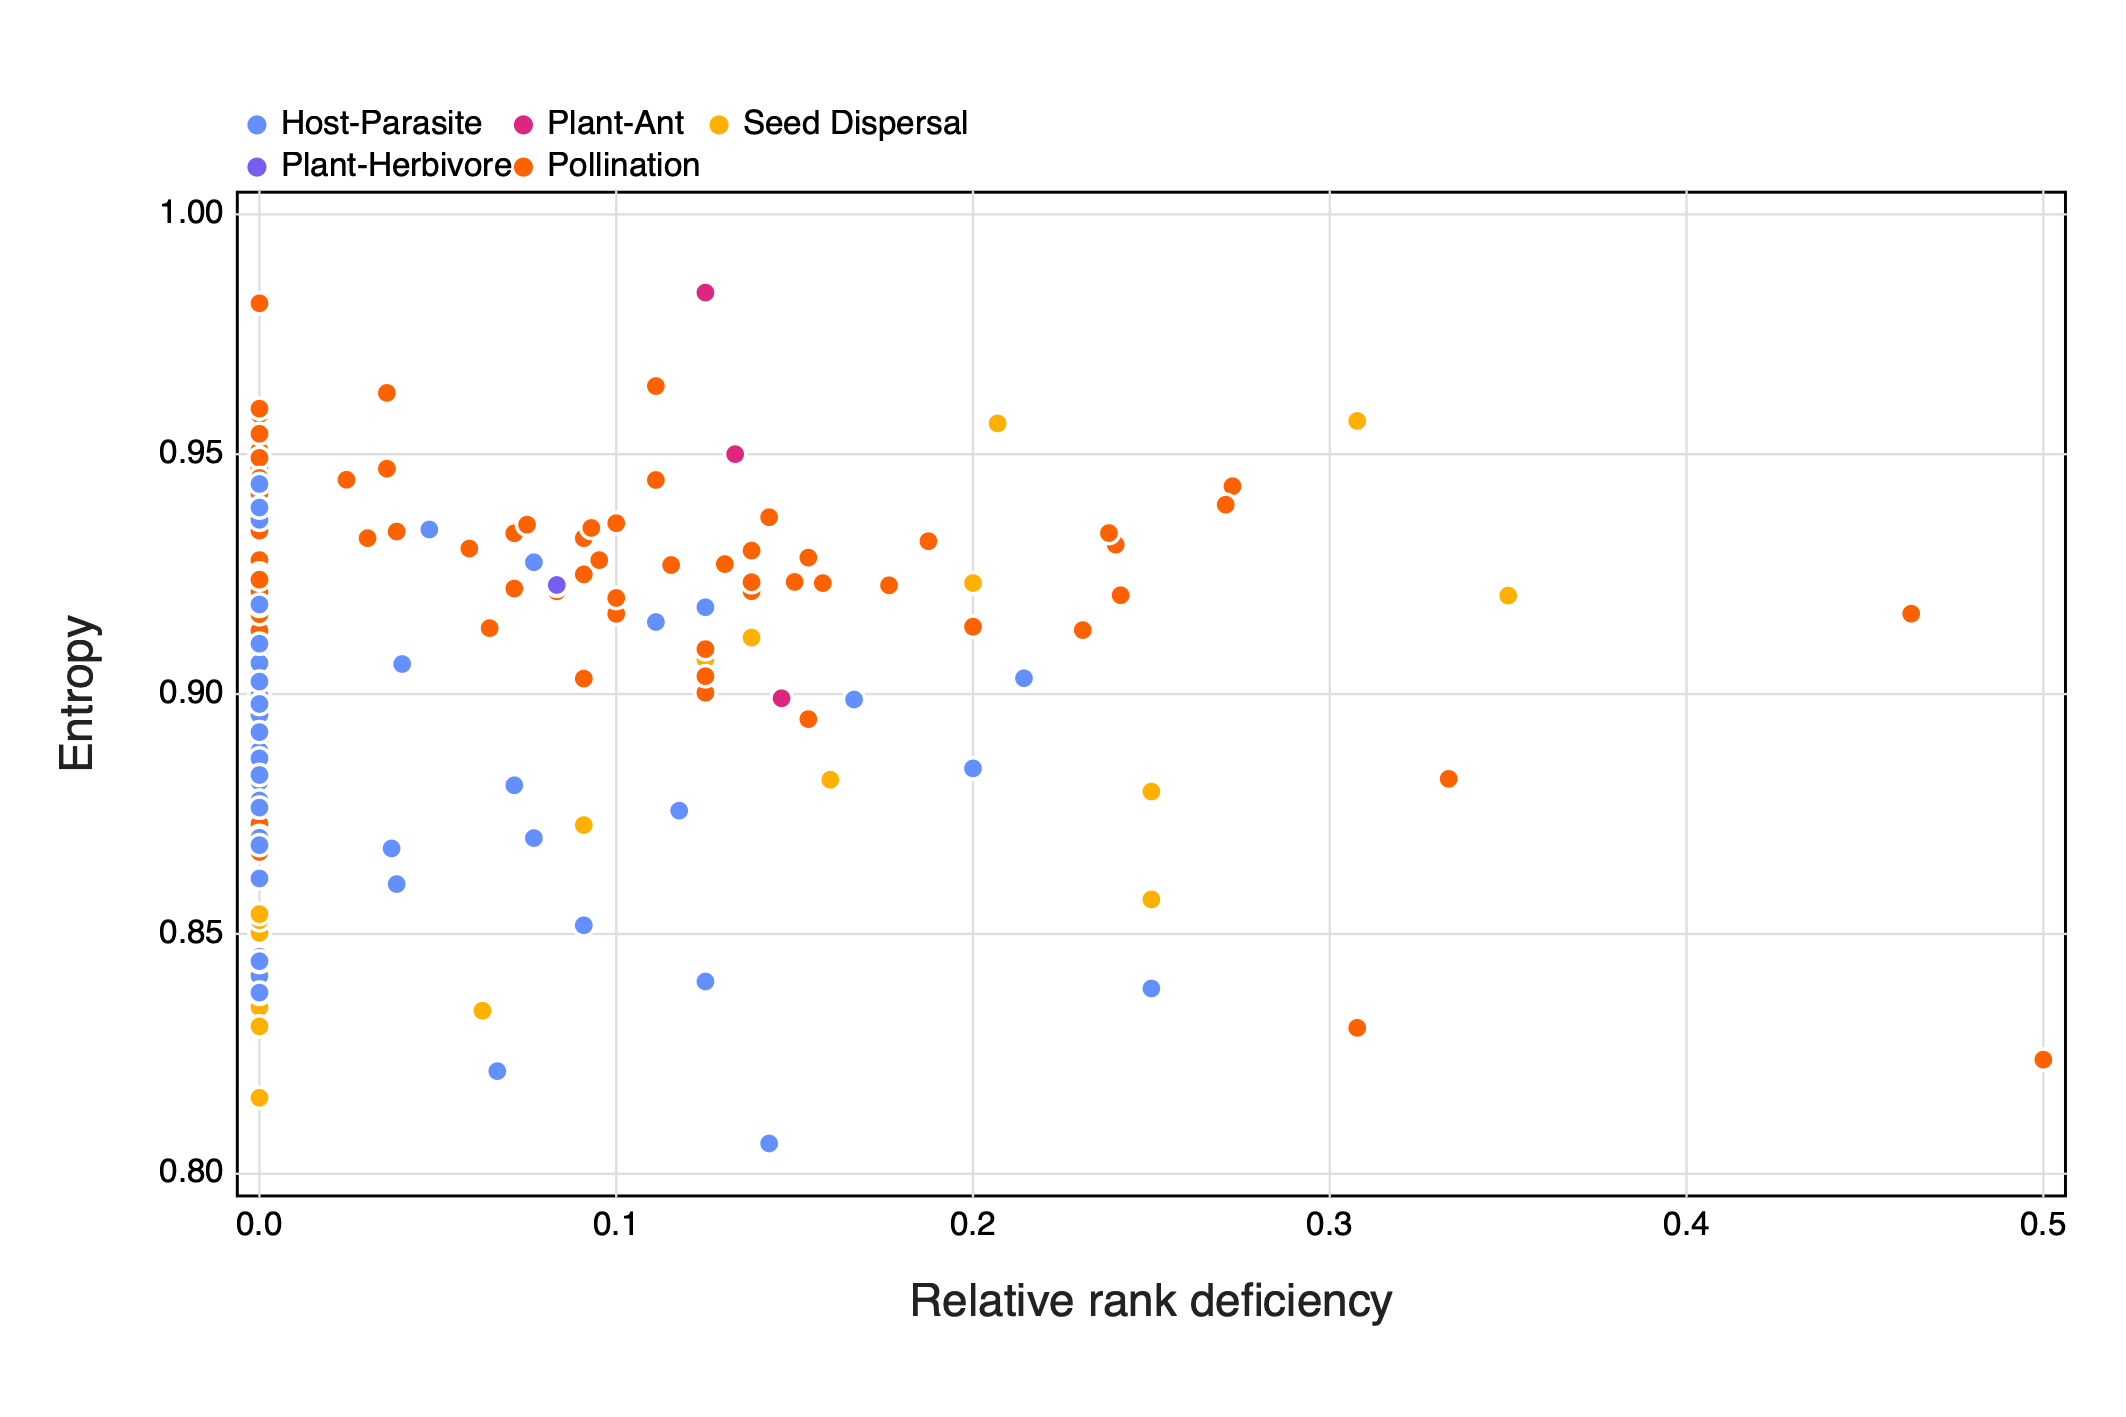
\includegraphics[width=\textwidth]{figures/entropy_v_rank.png}
    \caption{The relationship between SVD entropy and the relative rank
deficiency of different species interaction networks Colours indicate the
different interaction types of the networks.}
    \label{fig:entropy_v_rank}
\end{figure}

\subsection{Most elements of network structure capture network
complexity}\label{most-elements-of-network-structure-capture-network-complexity}

We compared SVD entropy to some of the more common measures of complexity,
namely nestedness (\(\eta\), as per \cite{Bastolla2009ArcMut}),
connectance (\(\text{Co}\)), and the spectral radius of the network (\(\rho\),
following \cite{Staniczenko2013GhoNes}). All of these measures are
positively correlated, especially over the range of connectances covered by
empirical bipartite ecological networks.

Nestedness is calculated based on the number of interactions shared between
species pairs and is a measure of the degree of overlap between species links
(or strategies) in the community, where larger assemblages are made up of a
subset of smaller ones that share common interactions. Networks with a higher
degree of nestedness could be considered simpler when compared to networks with
a lower degree of nestedness. Connectance is the realised number of interactions
(links) in an ecological network and is calculated as the fraction of the total
number of realised interactions (or links) and the maximum number of possible
interactions in a network (\cite{Martinez1992ConCon}). This has been shown to be a
good estimate of a community's resilience to perturbation
(\cite{Dunne2002NetStr}). The spectral radius of a matrix is the largest absolute
value of its eigenvalues, which, in addition to being presented as a measure of
network complexity has also been suggested as an indicator of the ability of a
system to dampen disturbances (\cite{Phillips2011StrEco}).

We find that SVD entropy has a clear negative relationship with nestedness,
spectral radius, and connectance (\autoref{fig:other}). As in
\autoref{fig:type}, mutualistic networks tend to be more complex, and they also
are both sparser and less nested than other types of networks.
\cite{Bastolla2009ArcMut} give a convincing demonstration that
mutualistic networks are shaped to minimise competition -- this can be done by
avoiding to duplicate overlap in interactions, thereby resulting in a network
that is close to full rank, and with high SVD entropy. Interestingly, \autoref{fig:other} suggests that both nestedness and connectance measure the \emph{lack} of complexity in an ecological network, which contrasts to how they may commonly be viewed (\cite{Landi2018Complexity}).

\begin{figure}[h]
    \centering
    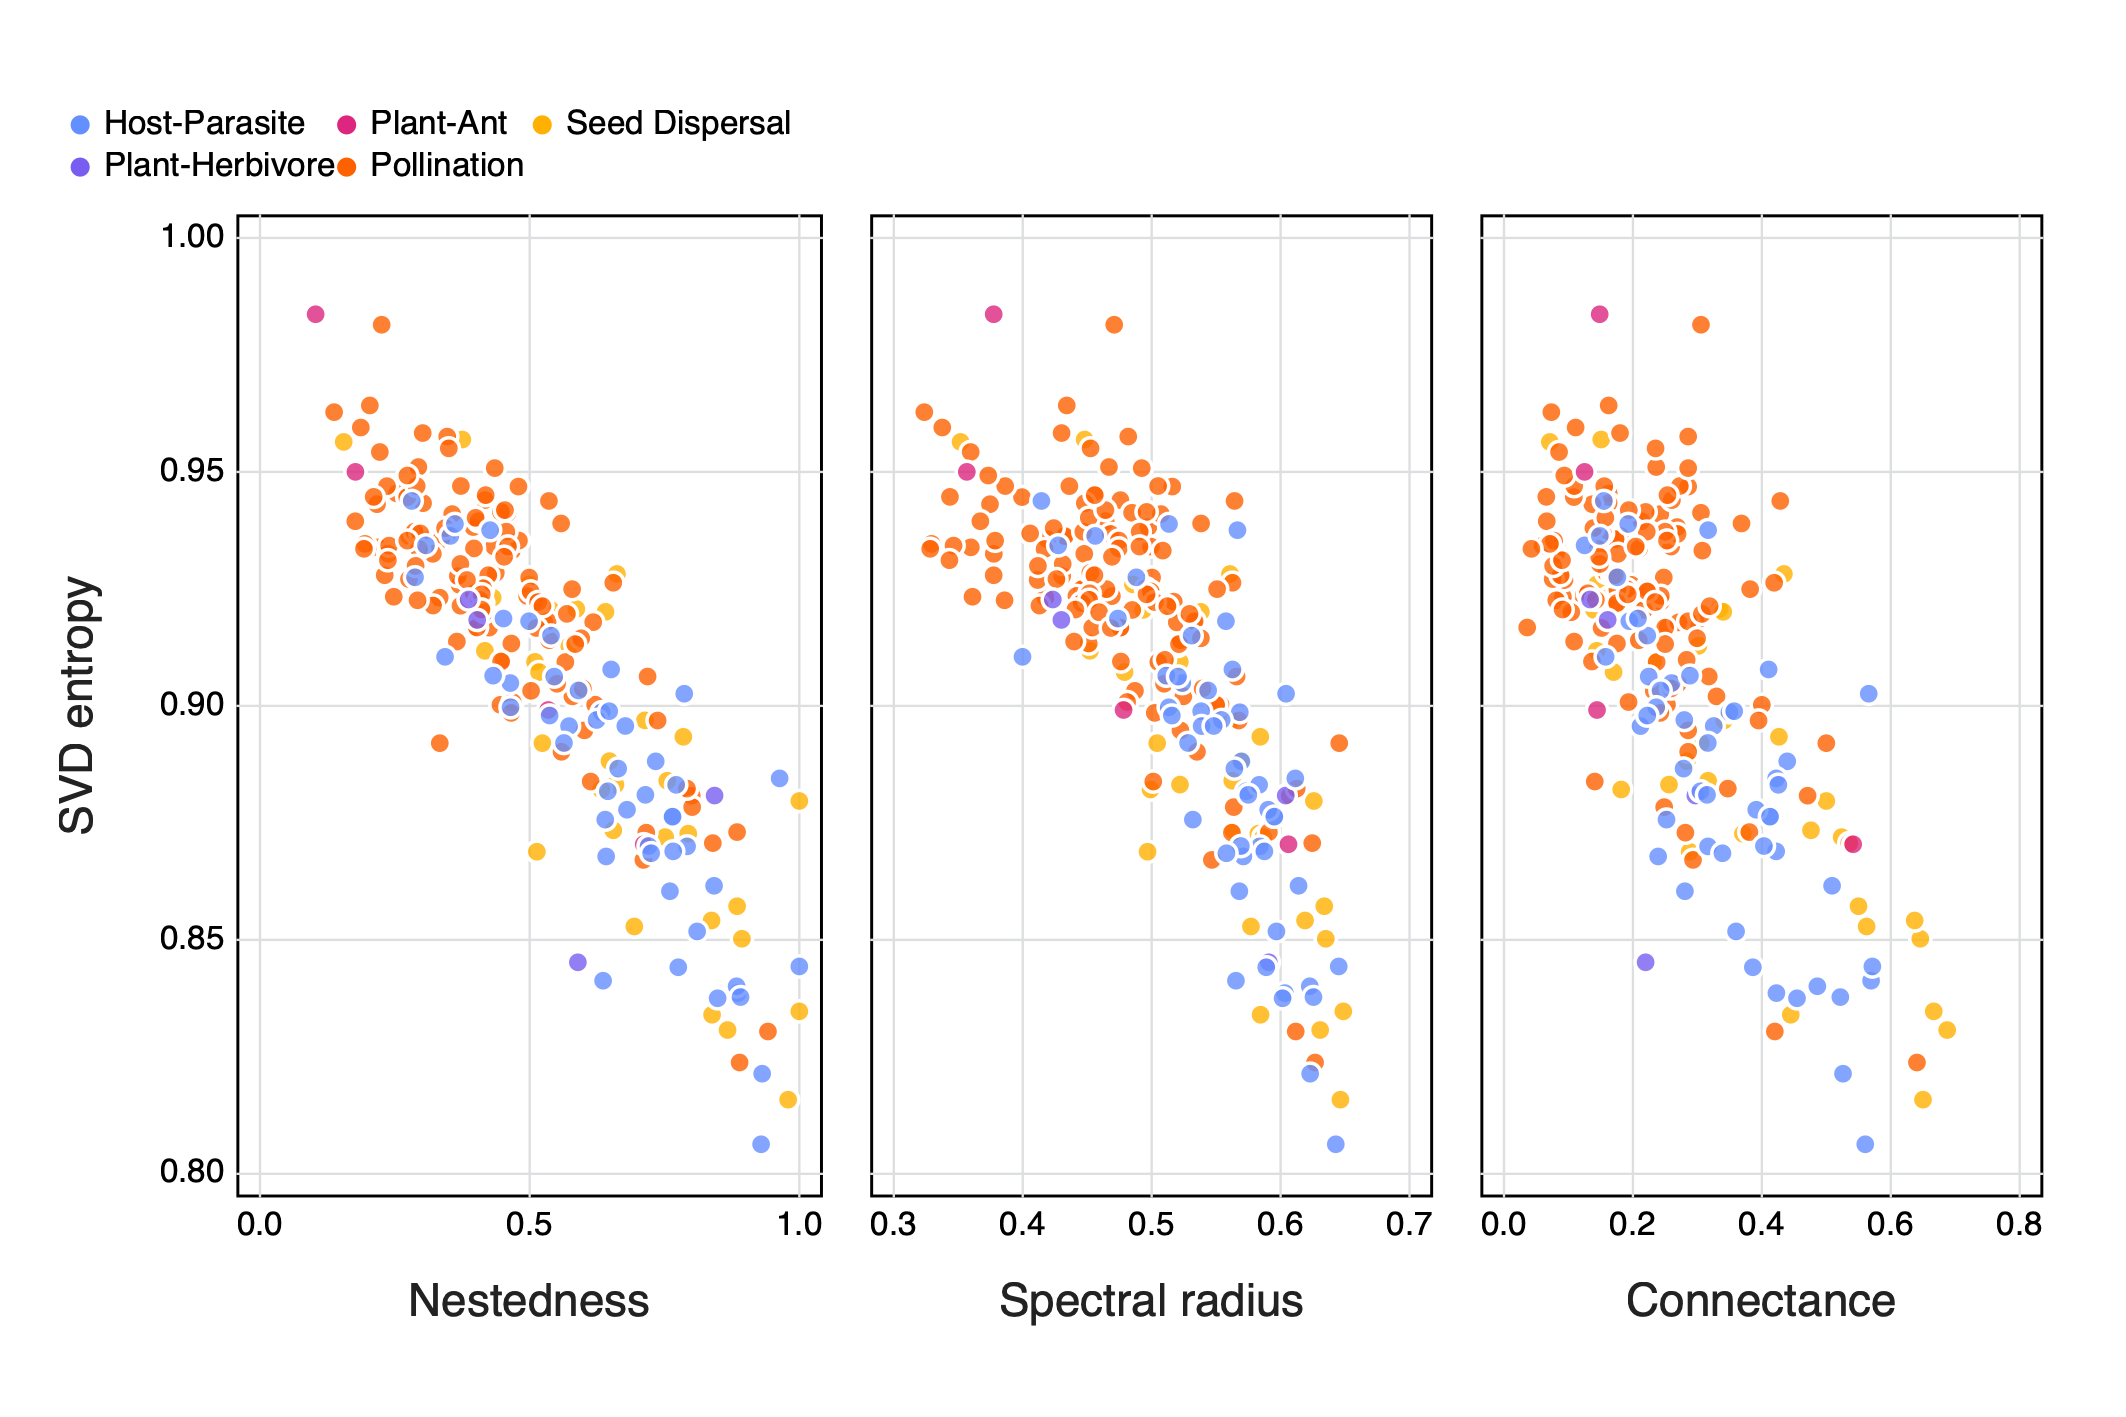
\includegraphics[width=\textwidth]{figures/others_v_entropy.png}
    \caption{The relationship between SVD entropy and the nestedness (left
panel), spectral radius (central panel) and connectance (right panel) of
ecological networks. Colours indicate the different interaction types of the
networks.}
    \label{fig:other}
\end{figure}

\subsection{Complex networks are not more robust to
extinction}\label{complex-networks-are-not-more-robust-to-extinction}

One approach to calculating the overall structural robustness of an ecological
network is by simulating extinction events through the sequential removal of
species, which allows constructing an extinction curve that plots the
relationship between species removed and cumulative secondary extinctions
(\cite{Dunne2002NetStr, Memmott2004TolPol}). Extinction events can be simulated in
a manner of different ways, either by removing 1) a random individual, 2)
systematically removing the most connected species (one with the highest number
of interactions with other species) and 3) the least connected species
(\cite{Dunne2002NetStr}). After each extinction event, we remove species from the
network that no longer have any interacting partners, thereby simulating
secondary extinctions. This is then repeated until there are no species
remaining in the network. Furthermore, we can restrict extinction events to only
one dimension of the interaction matrix, \emph{i.e.,} removing only top-level or
bottom-level species, or alternatively removing a species from any dimension of
the matrix. Extinction curves are then constructed by plotting the proportion of
species remaining against those that have been removed; it stands to reason that
a flatter curve `maintains' its species pool for a longer number of cumulative
extinctions, and could be seen as more resilient, when compared to a curve that
has a much steeper decline. As per previous studies, we measure the robustness
to extinction as the area under the extinction curve (AUC), calculated using the
Trapezoidal rule. AUC values close to 0 means that a single extinction is enough
to collapse the network almost entirely, and values close to 1 means that most
species persist even when the number of extinctions is really high.

When looking at the relationship between SVD entropy and the area under an
extinction curve (as a proxy for resilience to extinction) we find differences
depending on both the extinction mechanism as well as along which dimension the
species removal occurred (\autoref{fig:resilience}). As a whole we do not
observe any obvious relationships between SVD entropy and resilience, nor for
different interaction types. We do however see differences in the resilience of
networks depending on how the extinctions were simulated. Generally we see a
higher resilience in networks where species of only a specific group are removed
or in networks where species were either randomly removed or based on an
increasing number of interactions.

\begin{figure}[h]
    \centering
    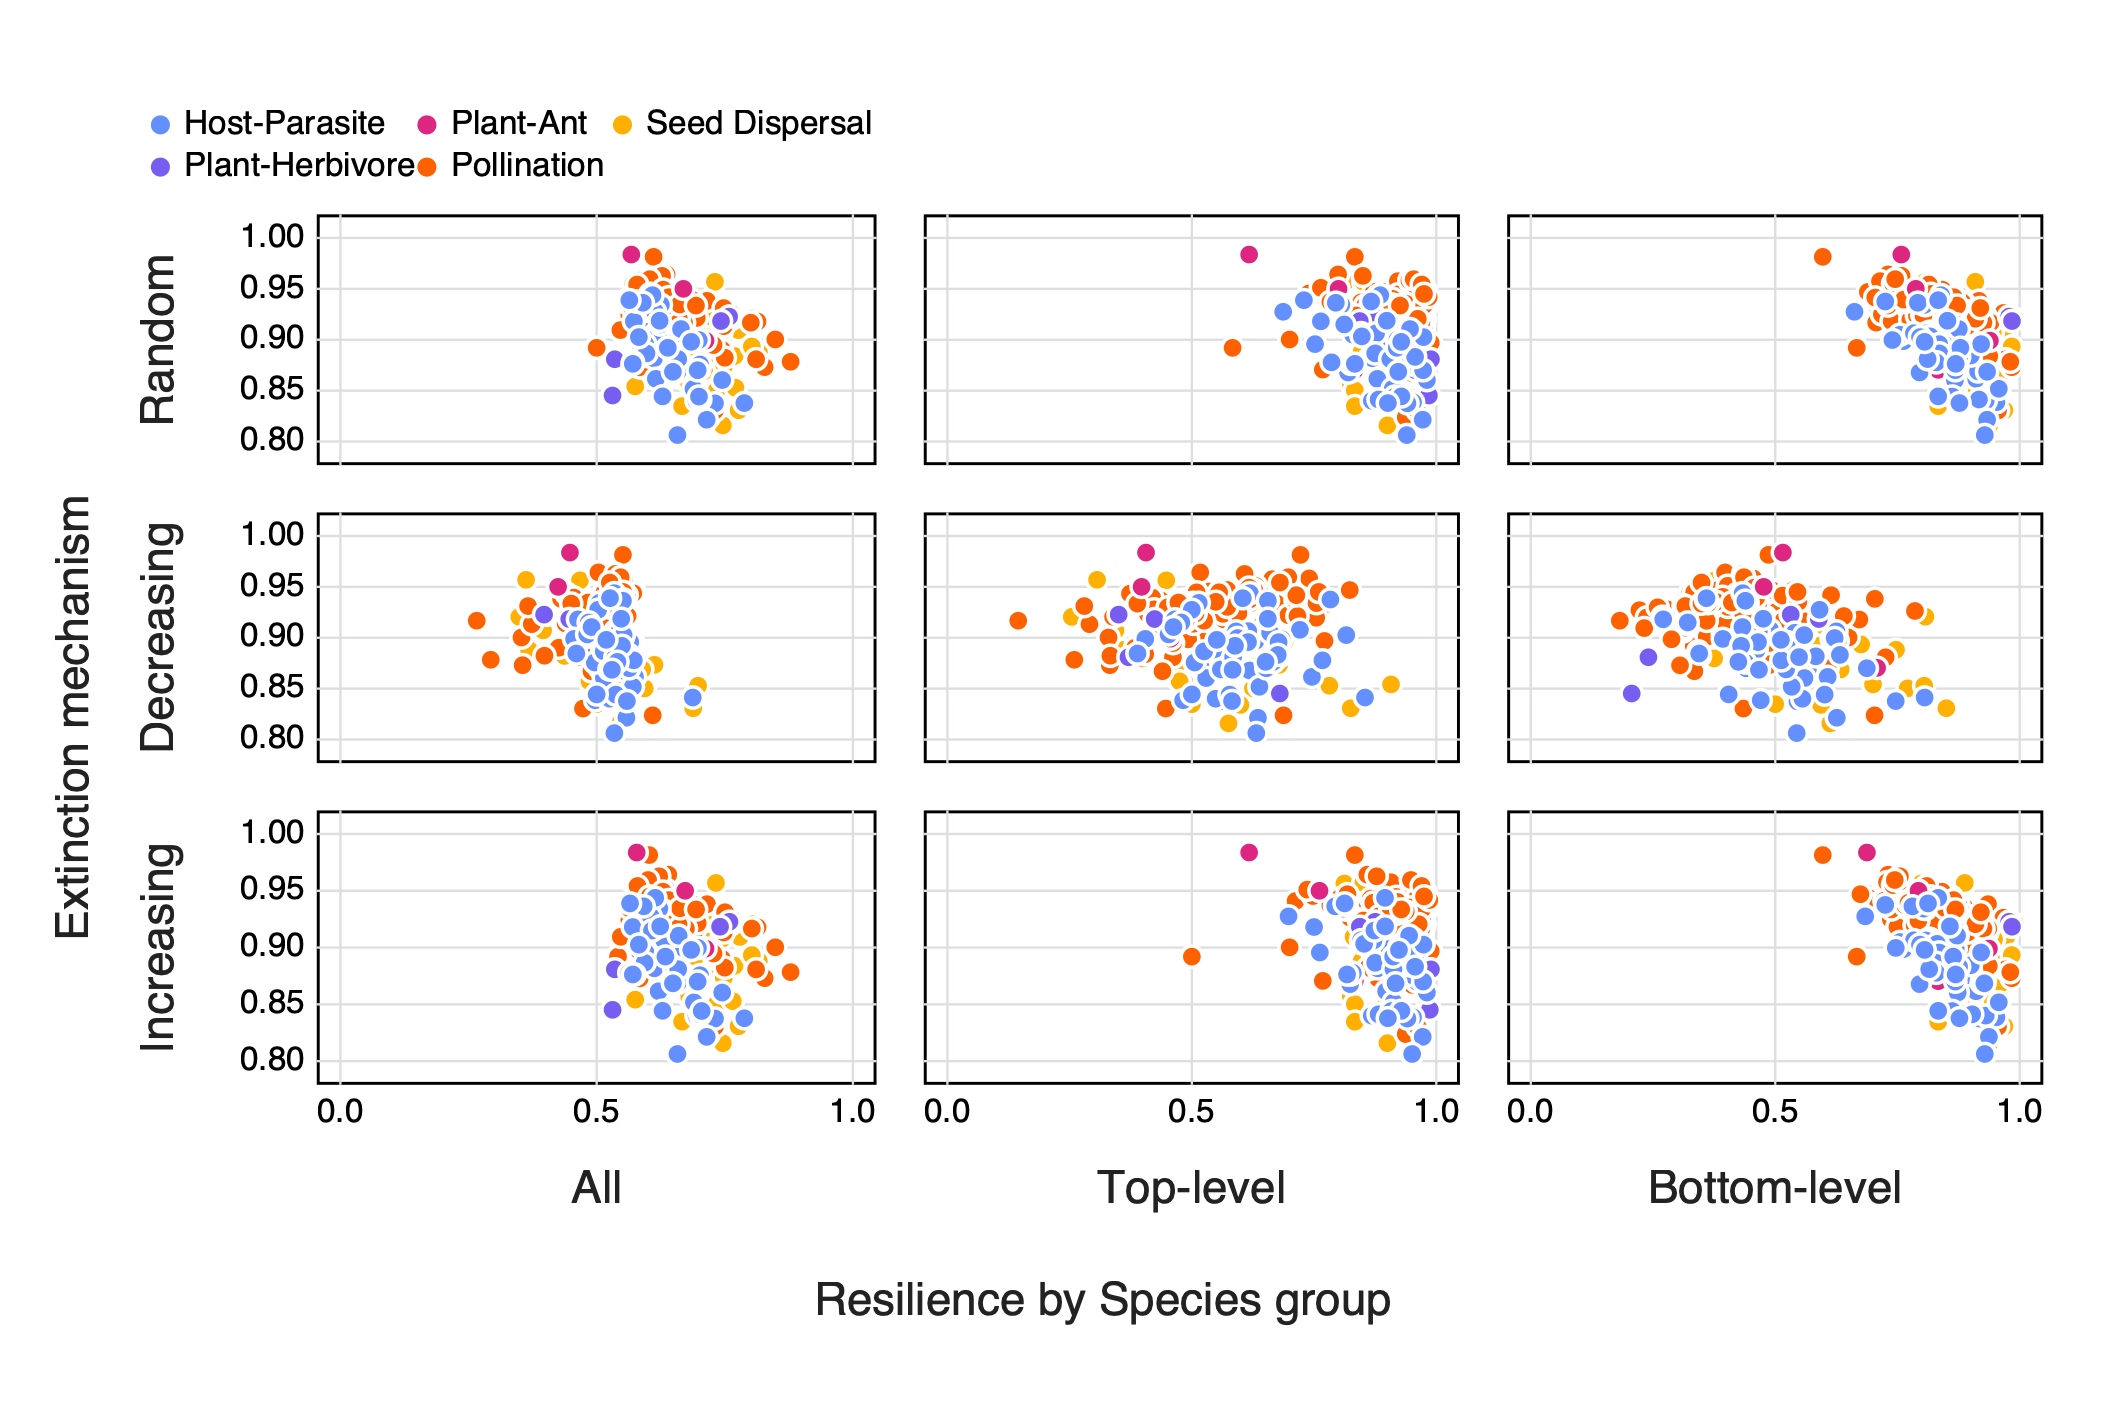
\includegraphics[width=\textwidth]{figures/entropy_v_AUCall.png}
    \caption{The relationship between SVD entropy and the area under an
extinction curve (as a proxy for resilience to extinction) for both different
extinction mechanisms (Random = the removal of a random species, Decreasing =
the removal of species in order of decreasing number of interactions (i.e most
to least number of interactions), Increasing = the removal of species in order
of increasing number of interactions) as well as along different dimensions
(species groups) of the network (All = any species, Top-level = only top-level
species, and Bottom-level = only bottom- level species) Colours indicate the
different interaction types of the networks.}
    \label{fig:resilience}
\end{figure}

As highlighted in \autoref{fig:other} SVD entropy can be used as an additional
measure of network complexity. However, as shown in \autoref{fig:resilience}, the
assumption that network complexity begets resilience to extinction begins to
unravel when we use a measure of physical complexity. This is in contrast to
previous studies that have shown how connectance plays a role in the resilience
of networks to extinctions (\cite{Dunne2002NetStr, Memmott2004TolPol}). This does
not discount the role of using \emph{structural} measures of network complexity
(\emph{e.g.,} connectance, nestedness or spectral radius) as indicators of their
resilience (although possibly hinting as to why there is no strong emerging
consensus as to how structural complexity relates to this), but rather points to
an erroneous assumption as to what aspects of a network we have previously used
to define its complexity.

\subsection{Plant-pollinator networks are slightly more
complex}\label{plant-pollinator-networks-are-slightly-more-complex}

Although we don't observe clear differences in the relationship between
different interaction types when comparing amongst various measures of
complexity, we do find that different types of interaction networks have
differing SVD entropy's. When comparing calculated SVD entropy between
interaction types using an ANOVA (after excluding Plant-Ant and Plant-Herbivore
interactions due to their small sample size in our dataset) we find a
significant difference between group means (\(F = 47.047, p < 10^{-3}\)). A
Tukey's HSD test reveals that plant-pollinator networks (\(\mu = .924\)) are
more complex than both host- parasite networks (\(\mu = .885, p < 10^{-3}\)) and
seed dispersal (\(\mu = .888, p < 10^{-3}\)). Host-parasite and seed dispersal
networks had apparently no difference in average complexity (\(p = .889\)).
These results suggest that mutualistic networks may be more complex, which
matches with previous literature: these networks have been shown to minimise
competition (\cite{Bastolla2009ArcMut}) and favour unique interactions, thereby
increasing network complexity. This specific structure can appear as a
side-process of either ecological (\cite{Maynard2018NetSpa}) or evolutionary
(\cite{Valverde2018ArcMut}) processes, but nevertheless leaves a profound imprint
on the complexity of the networks.

\begin{figure}[h]
    \centering
    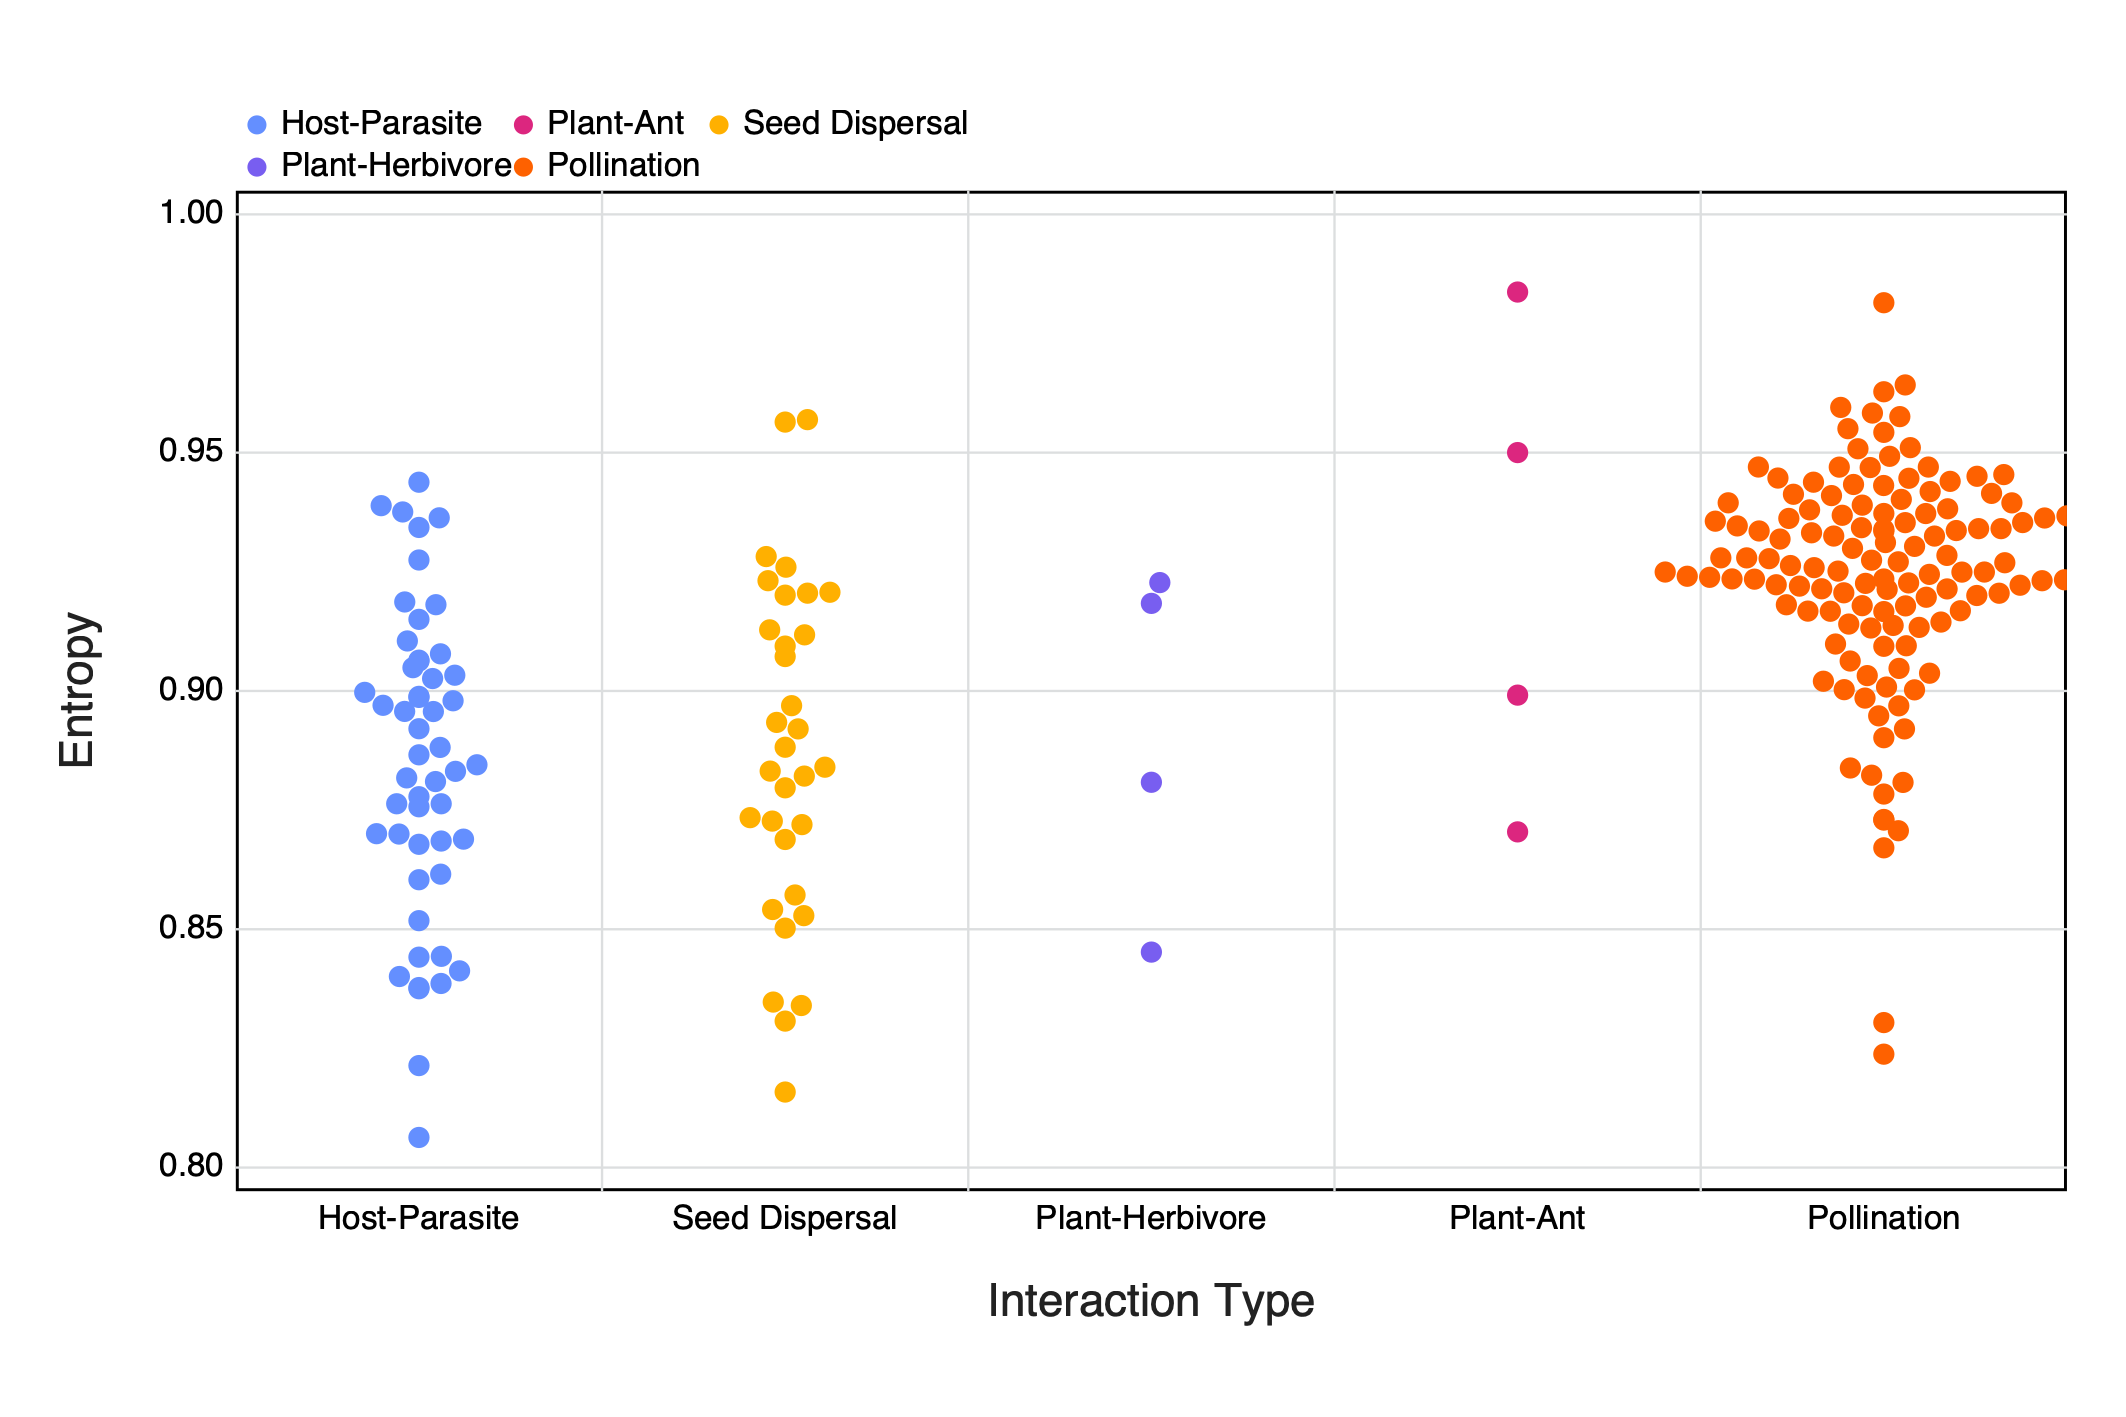
\includegraphics[width=\textwidth]{figures/interactiontype_v_entropy.png}
    \caption{The calculated SVD entropy of different interaction networks of
different interaction types}
    \label{fig:type}
\end{figure}

\subsection{Connectance constrains complexity (but also rank
deficiency)}\label{connectance-constrains-complexity-but-also-rank-deficiency}

We used simulated annealing (\cite{Kirkpatrick1984OptSim}) to generate networks
with the highest, or lowest, possible SVD entropy values. From a set network
size (30 species, 15 on each side) with a random number of interactions
(spanning the entire range from minimally to maximally connected), we
reorganised interactions until the SVD entropy was as close to 0 or 1 as
possible. We repeated the process 25 times for every number of interactions. We
also measured the relative rank deficiency of the generated networks. This
allows identifying the boundaries of both measures of complexity. The specific
simulated annealing we used is as follows. We set an initial temperature \(T_0 =
2\). At every timestep \(t\) (up until \(t = 10^4\)), the temperature is set to
\(T_t = T_0\times\lambda^t\), so that is decays exponentially at a rate
\(\lambda = 1 - 10^{-4}\). At each timestep, we switch two interactions in the
network \(\mathcal{N}\) at random to generate a proposal network
\(\mathcal{M}\). The score of this proposal is the difference between the
squared error of \(\mathcal{N}\) and \(\mathcal{M}\) \emph{i.e.,} \(\Delta =
(f(\mathcal{M})-\theta)^2-(f(\mathcal{N})-\theta)^2\), where \(f\) is the SVD
entropy and \(\theta\) is the target for optimisation (either 0 or 1 for
respectively minimally or maximally complex). A proposal is accepted with
probability \(\text{P}(\mathcal{N} \rightarrow \mathcal{M} | \Delta) =
\text{exp}\left(-\Delta\times T_t^{-1}\right)\).

By exploring the minimal and maximal values of SVD entropy for networks of a
given size, we can show that the range of complexity that a network can express
varies as a function of connectance (\autoref{fig:simann}). As reported by
\cite{Poisot2014WheEco}, there is no variation when the networks are
either minimally or maximally connected, but any connectance in between can give
rise to networks of varying complexities. This being said -- minimally connected
networks always show the largest complexity, and an increase in connectance will
always decrease complexity. Interestingly, this relationship is monotonous, and
there is no peak of complexity where the maximal number of possible networks
combination exists, \emph{i.e.,} around \(\text{Co} \approx 0.5\)
(\cite{Poisot2014WheEco}). This is an intriguing result -- ecological networks are
indeed extremely complex, but whereas ecologists have usually interpreted
connectance as a measure of complexity, it is in fact sparse networks that are
the complex ones, and connectance acts to decomplexify network structure.

\begin{figure}[h]
    \centering
    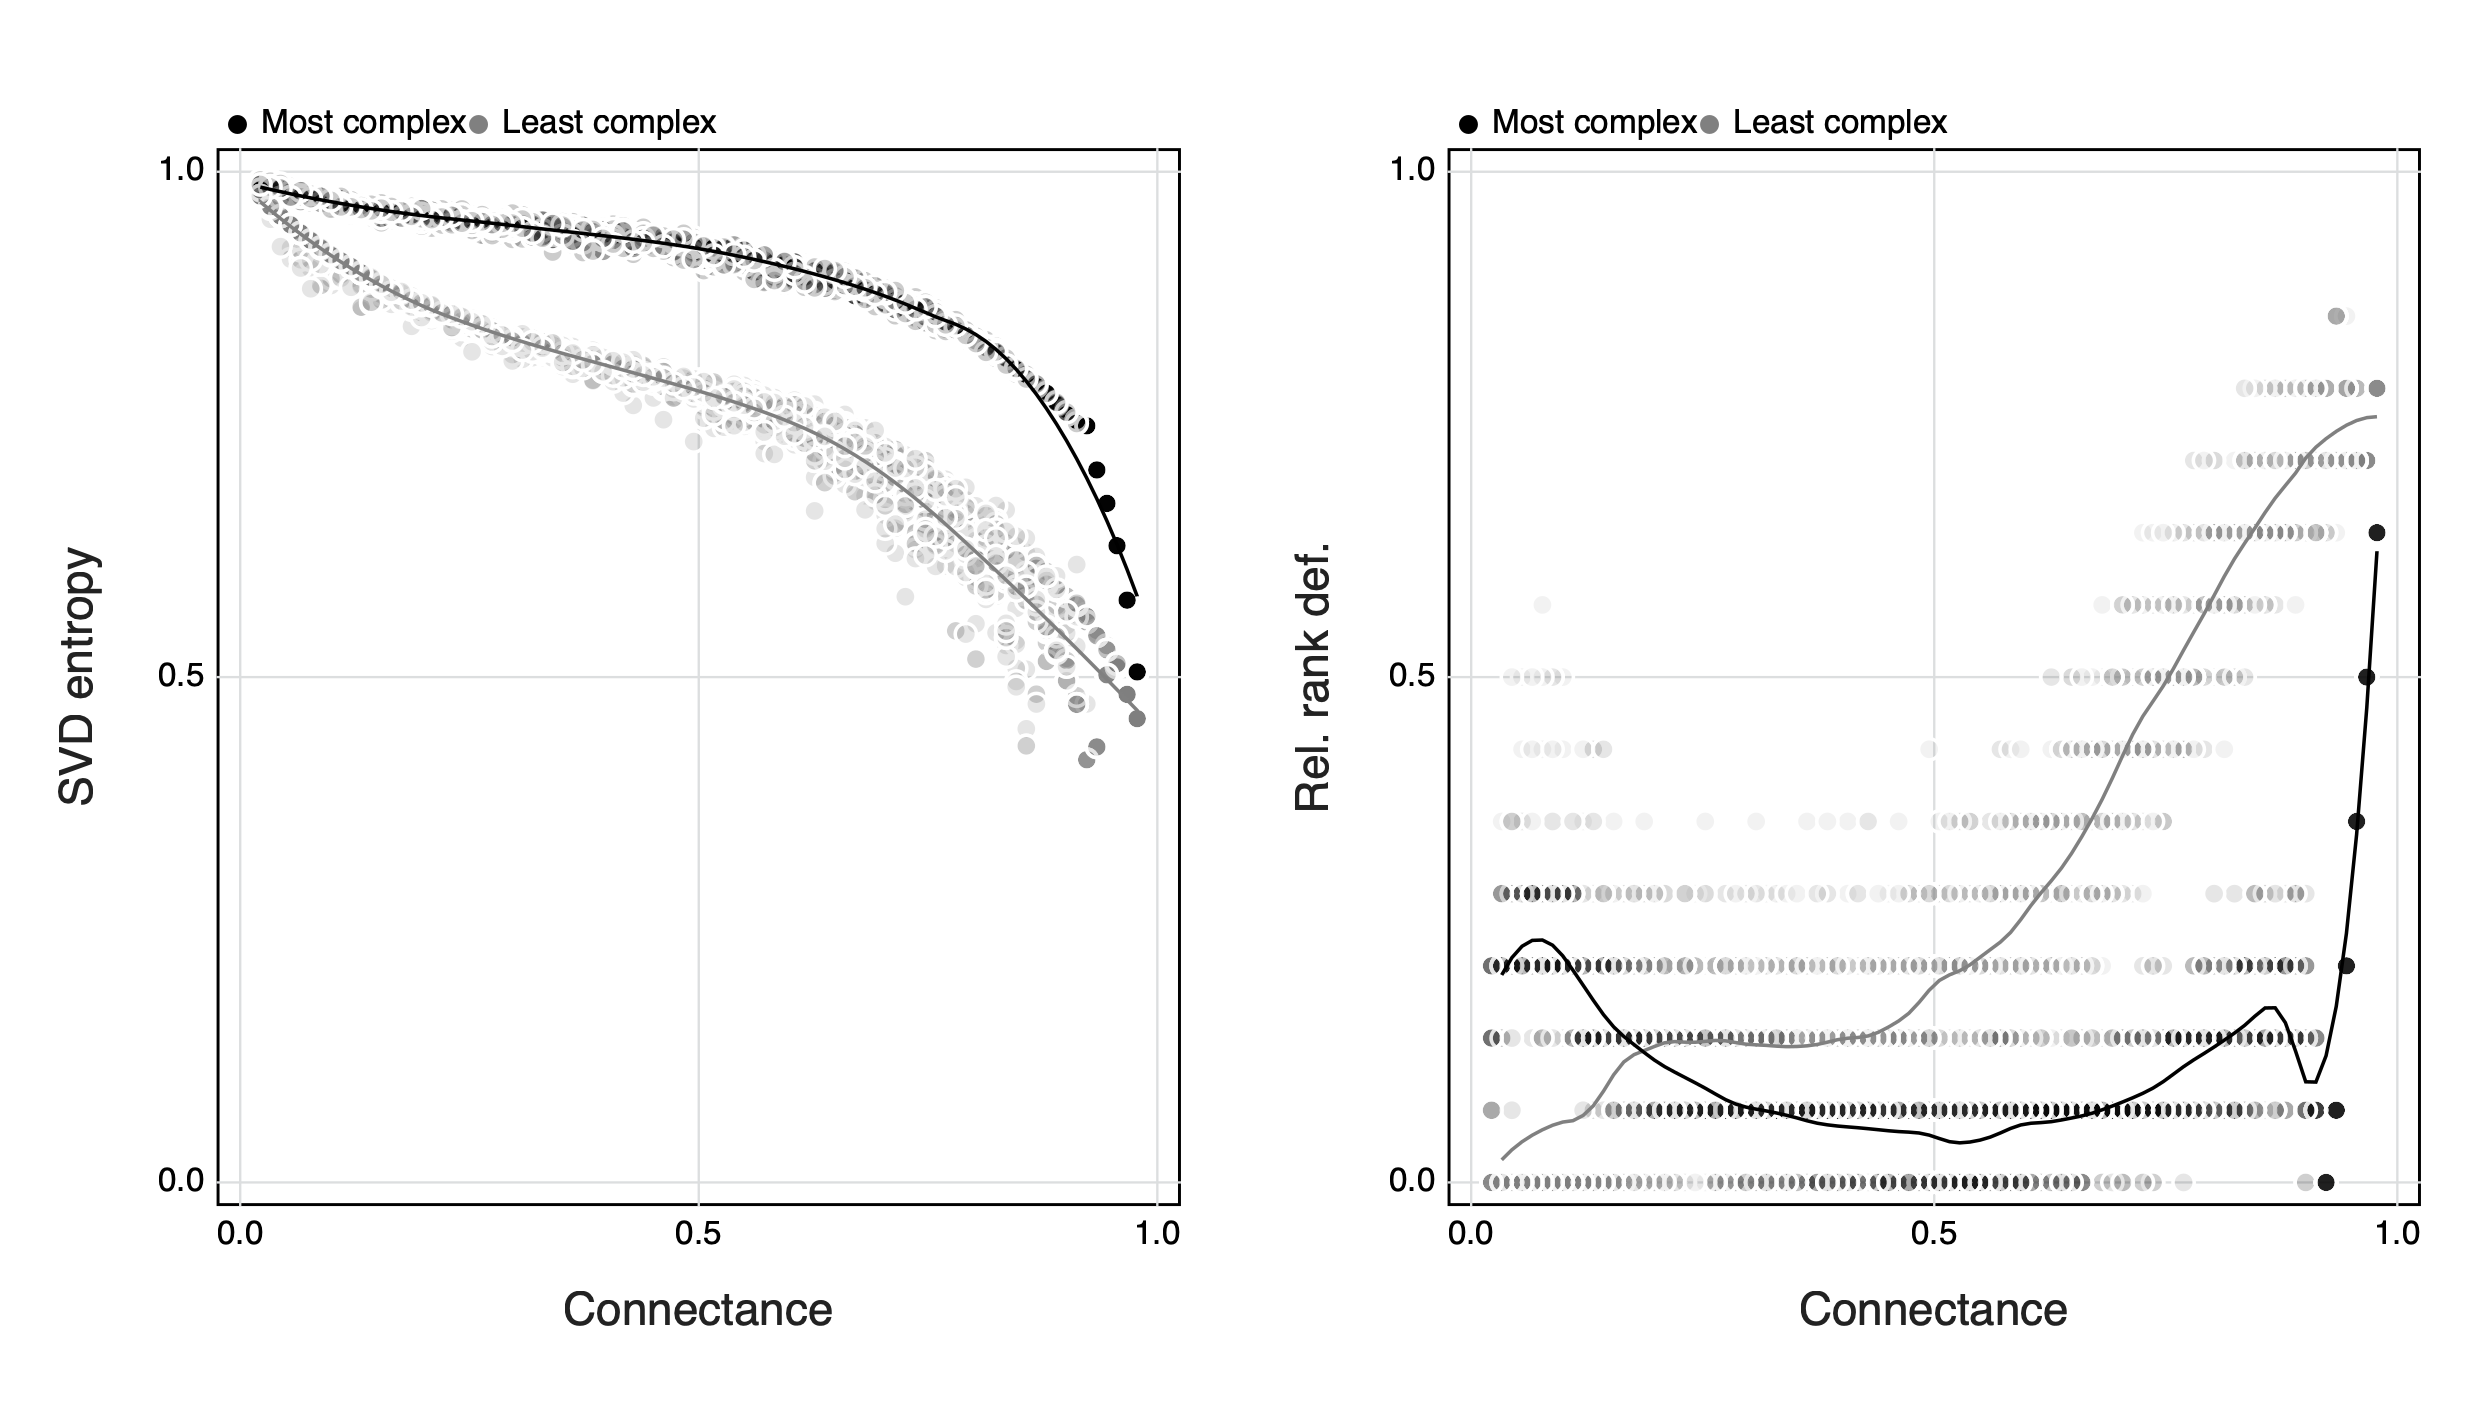
\includegraphics[width=\textwidth]{figures/minmax_combined.png}
    \caption{The relationship between the maximum and minimum value of SVD
entropy of a collection of random interaction networks (using simulated
annealing) for a given connectance spanning from 0 to 1 (left panel) and how
this relates to the relative rank deficiency of networks (right panel)}
    \label{fig:simann}
\end{figure}

The right panel of \autoref{fig:simann} shows the average rank deficiency of
networks for which SVD entropy was either maximised or minimised. Complex
networks (meaning, maximally complex given their connectance) had a lower
deficiency, indicating that except at extreme connectances, there are
combinations of networks for which all species can interact in unique ways --
this is a natural consequence of the results reported by
\cite{Poisot2014WheEco}, whereby the number of possible networks is only
really constrained at the far ends of the connectance gradient. Minimally
complex networks, on the other hand, saw their rank deficiency increase with
connectance. This hints at the fact that the decrease in complexity with
connectance may be primarily driven by the infeasibility of having enough
species for them to all interact uniquely as connectance increases. Because
non-unique interactions tend to result in competition
\cite{Bascompte2007PlaMut}, this can ``push'' networks towards the full-rank
configuration (as suggested by the results in \autoref{fig:size}), thereby
maximising complexity regardless of connectance.

\subsection{Larger networks are less complex than they could
be}\label{larger-networks-are-less-complex-than-they-could-be}

To assess whether ecological networks are more, or less, complex than expected,
we applied two null models that generate pseudo-random networks: Type I
(\cite{Fortuna2006HabLos}), where interactions happen proportionally to
connectance, and Type II (\cite{Bascompte2003Nested}), where interactions happen
proportionally to the joint degree of the two species involved. The models are
equivalent to, respectively, the Erdos-Renyi and Configuration models
(\cite{Newman2010NetInt}), both of which are maximum entropy generative models
that reflect global (Type I) or local (Type II) constraints
(\cite{Park2004Statistical}). We generated 999 samples for every network in the
dataset, and measured the \emph{z}-score of the empirical network as

\[z_i = \frac{x_i-\mu_i}{\sigma_i}\]\

where \(x_i\) is the SVD entropy of network \(i\), and \(\mu_i\) and
\(\sigma_i\) are respectively the average and standard deviation of the
distribution of SVD entropy under the null model. Negative values of \(z_i\)
reflect a network that has lower entropy than expected under the assumptions of
the null model. In \autoref{fig:nullmod}, we show that despite high
\emph{absolute} values of SVD entropy, ecological networks are not as complex as
they \emph{could} be. This is consistently true for both null models, and for
the three types of networks that had a sufficient sample size.

\begin{figure}[h]
    \centering
    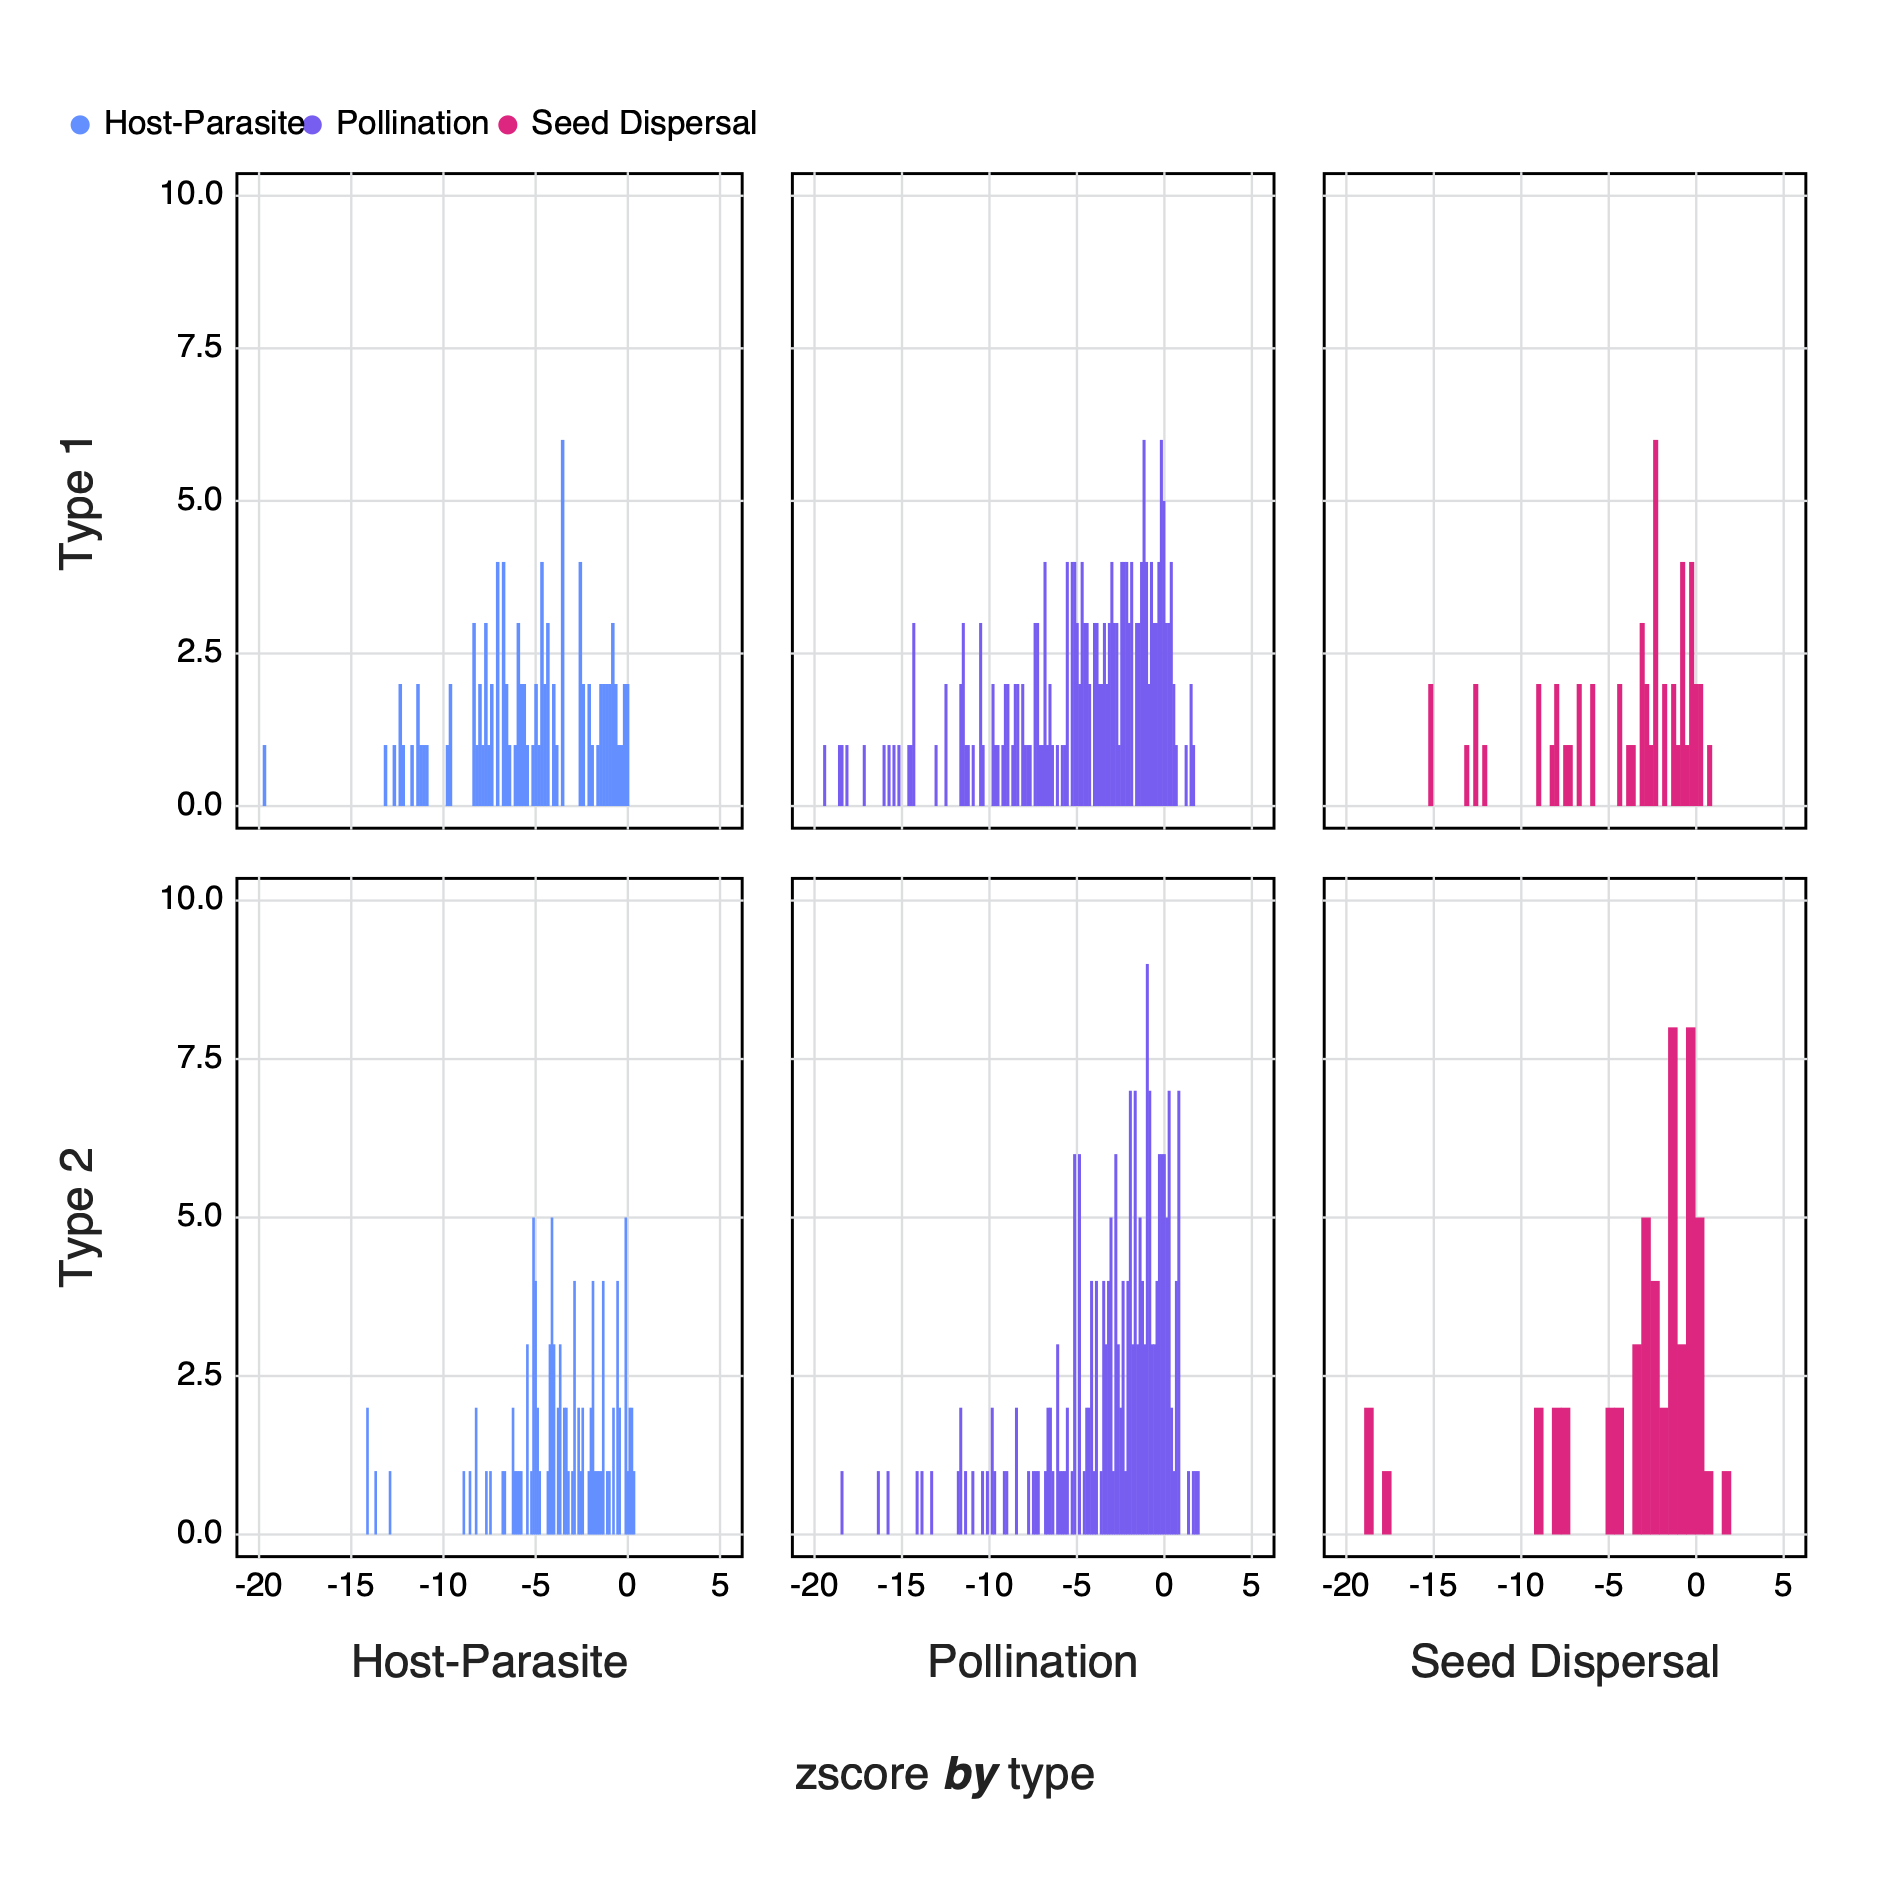
\includegraphics[width=\textwidth]{figures/nullmodel_histogram.png}
    \caption{The counts of the \(z_i\)-scores of different types of networks for
both Type I and Type II null models. Negative \(z_i\)-scores indicate networks
with an SVD entropy that is lower \emph{i.e.,} less complex than expected}
    \label{fig:nullmod}
\end{figure}

Previous work on random networks (using a model that is essentially the Type I
null model) shows that sufficiently large networks achieve maximal von Neuman
entropy (\cite{Du2010NotNeu, Passerini2011NeuEnt}). In \autoref{fig:larger}, we compare the
\emph{logistic} of \(z_i\) to the richness of the network. Transforming to the
logistic smooths out differences in absolute value that are apparent in
\autoref{fig:nullmod}, and projects the values in the unit range, with values
above \(0.5\) being more complex than expected. It is quite obvious that, across
both models and the three types of interactions, only smaller networks achieve
higher entropy. Both \cite{Barbier2018GenAss} and \cite{Saravia2018EcoNet} have previously noted that the early stages of
network assembly usually result in severely constrained networks, due to the
conditions required for multiple species to persist; as networks grow larger,
these constraints may ``relax'', leading in networks with more redundancy, and
therefore a lower complexity.

\begin{figure}[h]
    \centering
    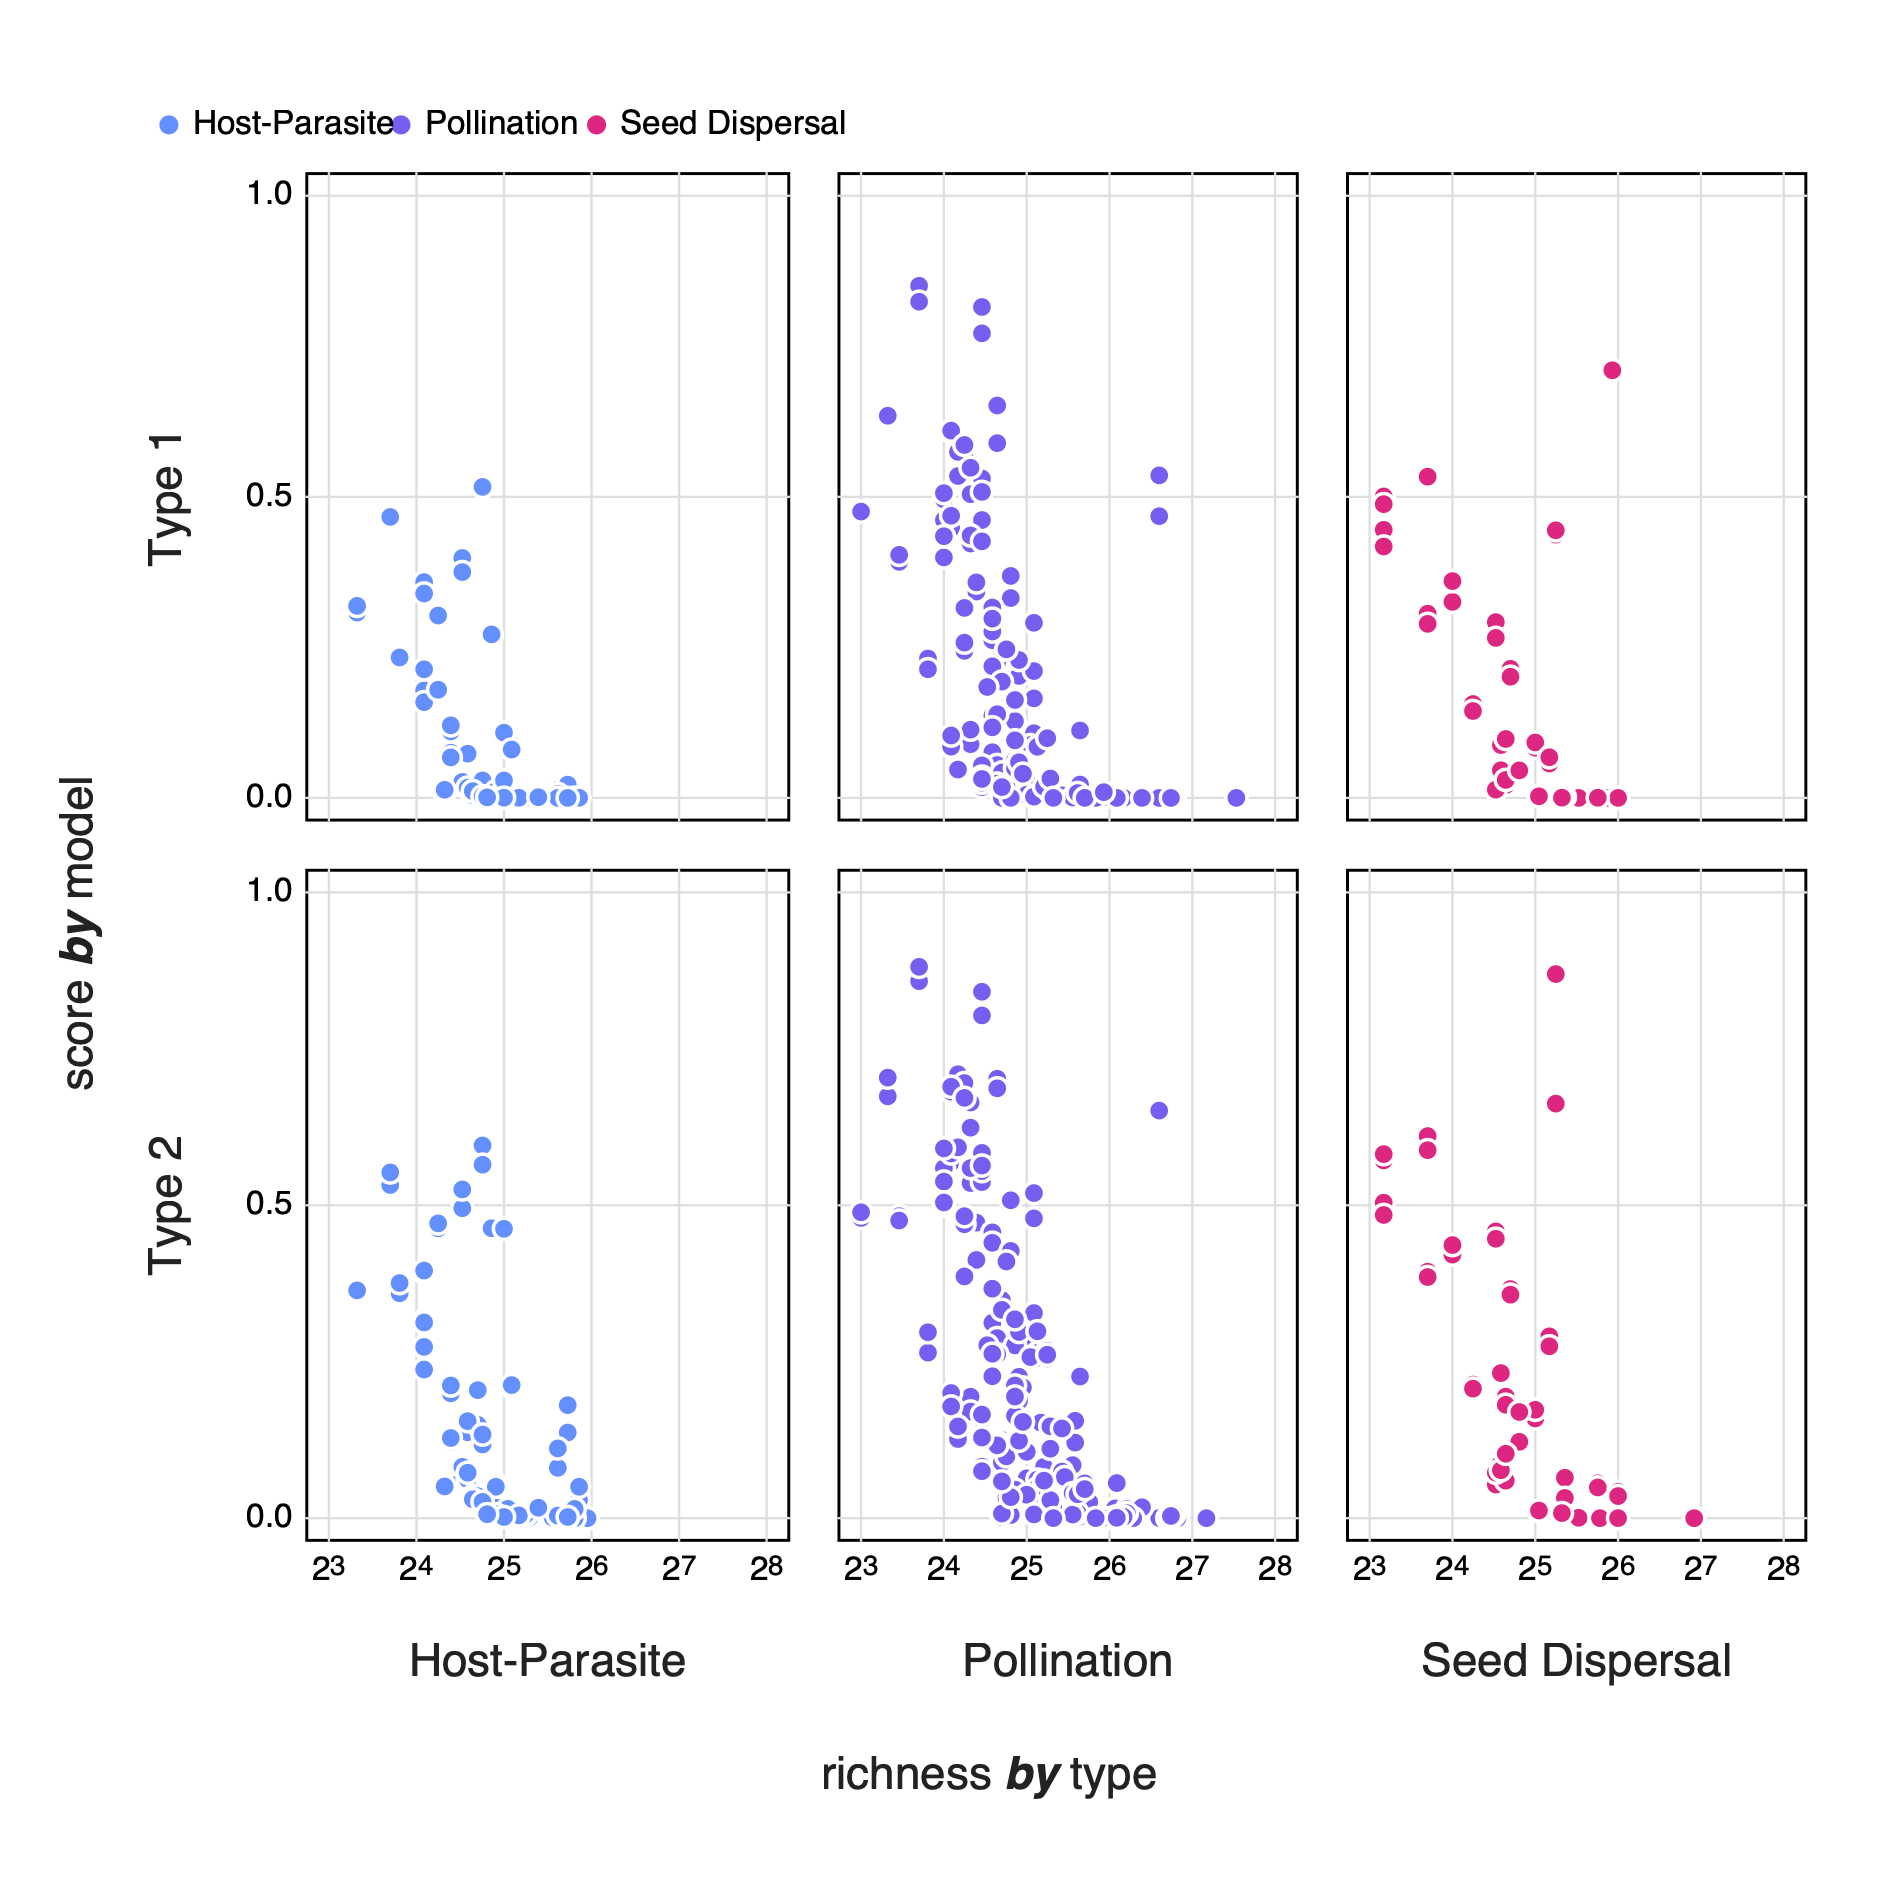
\includegraphics[width=\textwidth]{figures/nullmodel_richness.png}
    \caption{The logistic \(z_i\)-scores of different types of networks for both
Type I and Type II null models compared to the species richness of the network.
Where \(z_i\)-scores below 0.5 indicate networks with an SVD entropy that is
lower \emph{i.e.,} less complex than expected}
    \label{fig:larger}
\end{figure}

\clearpage

\section{Conclusion}\label{conclusion-svd}

We present SVD entropy as a starting point to unifying (and standardising) how
we should approach defining the complexity of ecological networks. The use of a
unified definition will allow us to revisit how complexity relates to the
ecological properties of networks using a standardised method. One important
result from using SVD entropy is that the complexity of ecological networks is
indeed \emph{immense}, yet despite this high complexity networks are still not
reaching their \emph{maximum} potential complexity. We suggest that the assembly
dynamics of networks may explain this observation but this still raises the
question as to why larger (or more mature) networks are not `maintaining' their
expected complexity and prompts further exploration as to the role of ecological
assembly in structuring networks.

\printbibliography{}
\end{refsection}

\endinput
%%
%% End of file `article1.tex'.
